\chapter{Desarrollo del TFG}
\label{ch:desarrollo}

\section{Metodología de Trabajo}
\label{sec:Metodologia}

La metodología empleada para el desarrollo de este Trabajo de Fin de Grado se basa en el Diseño Basado en Modelos (\gls{MBD}), combinado con un enfoque de prototipado iterativo. Dada la elevada complejidad matemática que rige la coordinación de la cinemática paralela junto con las estrictas restricciones geométricas impuestas por la trayectoria solar, resulta inviable abordar la construcción directa de un prototipo físico sin una validación teórica exhaustiva.

El uso de esta metodología garantiza que cualquier decisión de diseño mecánico se haya tomado con una previa verificación de su viabilidad, minimizando los riesgos de fallo, el desperdicio de material y los costes de fabricación. De esta forma, el desarrollo del Trabajo de Fin de Grado se ha estructurado según el proceso descrito en el diagrama de flujo de la Figura \ref{fig:diagrama_metodologia}

\tikzstyle{startstop} = [rectangle, rounded corners, 
minimum width=3cm, 
minimum height=1cm,
text centered, 
draw=black, 
fill=red!30]

\tikzstyle{process} = [rectangle,
minimum width=3cm, 
minimum height=1cm,
text width=6cm, 
text centered,
draw=black, 
fill=orange!30]

\tikzstyle{decision} = [diamond, 
minimum width=1cm, 
minimum height=1cm, 
text centered, 
draw=black, 
fill=green!30]

\tikzstyle{arrow} = [thick,->,>=stealth]
\begin{figure}[H]
\centering
\begin{tikzpicture}[node distance=2cm]

\node (start)  [startstop] {Definición del objetivo del proyecto};
\node (MAA)    [process, below of=start] {Modelado Analítico y Algorítmico};
\node (CVV)    [process, below of=MAA] {Cosimulación y Validación Virtual};
\node (dec1)   [decision, below of=CVV, yshift=-0.5cm,
    label={[align=right]left:¿Cumple\\requisitos?}]{};
\node (pro2a)  [process, below of=dec1, yshift=-0.5cm] {Materialización e Integración Mecatrónica};
\node (pro2b)  [process, right of=dec1, xshift=3cm] {Síntesis y Rediseño Iterativo};
\node (stop)   [startstop, below of=pro2a] {Validación Empírica de Campo};

\draw [arrow] (start)  -- (MAA);
\draw [arrow] (MAA)    -- (CVV);
\draw [arrow] (CVV)    -- (dec1);
\draw [arrow] (dec1)   -- node[anchor=east]  {sí} (pro2a);
\draw [arrow] (dec1)   -- node[anchor=south] {no} (pro2b);
\draw [arrow] (pro2b)  |- (CVV);
\draw [arrow] (pro2a)  -- (stop);

\end{tikzpicture}
\caption{Diagrama de flujo de la metodología empleada}
\label{fig:diagrama_metodologia}
\end{figure}

\subsection{Definición del objetivo del proyecto}
La fase inicial del proceso consiste en delimitar el problema y fijar los requisitos que debe satisfacer el sistema de seguimiento solar. A partir del objetivo del proyecto (Capítulo~\ref{ch:objetivos}), se establecen las condiciones que la arquitectura robótica ha de cumplir: mantener la lente de Fresnel perpendicular al sol conservando un punto focal estático, y disponer de la rigidez, la precisión y el rango angular necesarios para acompañar la trayectoria solar útil a lo largo del año en la latitud de Toledo. Estos requisitos constituyen la entrada que guía las etapas posteriores del desarrollo.

\subsection{Modelado Analítico y Algorítmico}
La primera etapa consiste en la abstracción matemática del problema. Comprende la formulación de las ecuaciones de cinemática inversa mediante matrices de rotación tridimensionales y el desarrollo del software base en Python, incluyendo el algoritmo de visión artificial para el cálculo del vector de error.

\subsection{Cosimulación y Validación virtual}
Como siguiente paso en el proyecto, se modela virtualmente el robot paralelo elegido en SolidWorks (creación de un gemelo digital). Simultáneamente, se implementa el modelo matemático de su cinemática inversa para gobernar los actuadores del modelo 3D, lo que permite mapear y simular su espacio de trabajo efectivo.

Una vez determinadas las limitaciones espaciales de la arquitectura, se somete a una validación cinemática superponiéndolo con las trayectorias solares locales correspondientes a fechas astronómicas críticas (solsticios y equinoccios). Este proceso de verificación virtual sirve como un criterio de viabilidad, el análisis determina si la arquitectura mecánica posee la amplitud angular exigida para aprovechar el ciclo solar de forma deseada.

\subsection{Síntesis y Rediseño Iterativo}
Basándose en los resultados obtenidos en la fase de simulación, la metodología exige un retorno a la fase de diseño si no se cumplen los requisitos. Fue en esta etapa donde se descartó la arquitectura Gough-Stewart clásica. En su lugar se sintetiza una arquitectura híbrida formada por dos mecanismos planos de lazo cerrado cinemáticamente desacoplados, uno por cada eje de orientación: una cadena de seis barras tipo Stephenson III para el movimiento acimutal y un mecanismo biela-manivela para el movimiento cenital. El nuevo conjunto se reincorpora al flujo metodológico, repitiendo la fase de cosimulación y validación virtual hasta verificar que su espacio de trabajo cubre las trayectorias solares requeridas.

\subsection{Materialización e Integración Mecatrónica}
Validada cinemáticamente una arquitectura que satisface los requisitos, el modelo se materializa en un sistema mecatrónico real. Esta fase comprende la integración del hardware electrónico y el desarrollo del software del bucle de control, repartido entre tres nodos comunicados por una red WiFi local autónoma: un nodo de visión, un nodo de control y una estación de supervisión. La fabricación y el ensamblaje del prototipo mecánico a escala real se desarrollan en paralelo por el grupo de investigación MANTIS, por lo que quedan fuera del alcance directo de este Trabajo.

\subsection{Validación Empírica de Campo}
La última fase del proceso consiste en verificar el funcionamiento del sistema completo en condiciones reales de operación, sometiendo el prototipo físico a un ciclo solar y contrastando su comportamiento con el previsto en la fase de simulación. Esta validación experimental sobre el prototipo a escala real corresponde al grupo de investigación MANTIS, conforme al reparto de tareas acordado; el presente Trabajo le proporciona los modelos, algoritmos y software validados de forma teórica y virtual sobre los que apoyar esta etapa.

\section{Modelado Analítico y Algorítmico}
Establecido el marco metodológico general, esta sección aborda la primera fase troncal del proyecto: la abstracción matemática y lógica del problema físico. El objetivo del modelado analítico y algorítmico es dotar al sistema de seguimiento visual capaz de detectar la posición exacta del Sol y de un modelo matemático que traduzca esa información en instrucciones de movimiento. El desarrollo de esta fase se divide en dos grandes bloques interdependientes que conforman el lazo de control del sistema. En la figura \ref{fig:diagrama_control} se muestra un diagrama de bloques que representa el bucle de control usado.


\tikzstyle{block} = [rectangle, rounded corners,
minimum width=3cm, minimum height=1cm,
text centered, draw=black, fill=orange!20]

\tikzstyle{block} = [rectangle, rounded corners,
minimum width=2.5cm, minimum height=1cm,
text centered, text width=2.5cm,
draw=black, fill=orange!20]

\tikzstyle{sensor} = [rectangle, rounded corners,
minimum width=2.5cm, minimum height=1cm,
text centered, text width=2.5cm,
draw=black, fill=blue!20]

\tikzstyle{sum} = [circle, minimum size=0.7cm, draw=black, fill=white]

\tikzstyle{arrow} = [thick,->,>=stealth]

\begin{figure}[H]
\centering
\begin{tikzpicture}[node distance=2cm, auto]

% Fila superior
\node (sol)     [block, fill=yellow!40]                {Posición solar};
\node (sum)     [sum,   right of=sol,  xshift=0.8cm]   {$\Sigma$};
\node (CIK)     [block, right of=sum,  xshift=1.5cm]   {Cinemática inversa};
\node (stewart) [block, right of=CIK,  xshift=2cm]     {Plataforma Gough-Stewart};

% Fila inferior
\node (proc) [sensor, below of=CIK, yshift=0cm, xshift=0cm] {Procesamiento de imagen};

% Puntos de giro auxiliares
\coordinate (A) at (stewart.south |- proc.east);  % mismo nivel que proc, bajo stewart
\coordinate (B) at (sum.south     |- proc.west);  % mismo nivel que proc, bajo sum

% Cadena directa
\draw [arrow] (sol)     -- node[above] {$\theta_{ref}$} (sum);
\draw [arrow] (sum)     -- node[above] {$e$}            (CIK);
\draw [arrow] (CIK)     -- node[above] {$l_i$}          (stewart);

% Plataforma baja hasta nivel de proc, luego va a proc
\draw [arrow] (stewart.south) -- (A) -- node[above] {posición} (proc.east);

% proc va a la izquierda hasta bajo el sumador, luego sube al sumador
\draw [arrow] (proc.west) -- (B) -- (sum.south);

% Signos del sumador
\node [above left=0.05cm of sum] {\small $+$};
\node [below right=0.05cm     of sum]  {\small $-$};

\end{tikzpicture}
\caption{Diagrama de bloques del bucle de control de la primera arquitectura}
\label{fig:diagrama_control}
\end{figure}

\subsection{Procesamiento de imagen y cálculo de error de apuntamiento}
\label{sec:procesamiento_imagen}

A continuación se explica el desarrollo y funcionamiento del sistema de visión artificial desarrollado para la detección y seguimiento del sol. Su función principal es, a partir de cada fotograma capturado por la cámara, determinar con precisión la posición del centroide solar en el plano imagen y traducir dicho desplazamiento en magnitudes angulares que el sistema de control pueda utilizar para corregir la orientación del seguidor.

\subsubsection{Inicialización del sistema de captura}

La adquisición de imagen se realiza mediante la biblioteca OpenCV, utilizando el objeto \texttt{VideoCapture}, también se emplea el backend \texttt{CAP\_DSHOW} (DirectShow), que reduce significativamente la latencia en la inicialización.

Junto con la apertura del dispositivo, se leen las dimensiones nativas del sensor \\\texttt{CAP\_PROP\_FRAME\_HEIGHT} y \texttt{CAP\_PROP\_FRAME\_WIDTH}, que se almacenan como parámetros globales. Estos valores son imprescindibles para dos operaciones posteriores: el cálculo del centro óptico de la cámara y la conversión de distancias en píxeles a ángulos reales.

\subsubsection{Parámetros del Modelo de Cámara: Campo de Visión}
El modelo geométrico adoptado asume una proyección en perspectiva con campo de visión \gls{FOV} conocido. Se definen dos parámetros angulares:
\begin{itemize}
    \item \gls{FOV} horizontal: representa el barrido angular del plano horizontal y el plano imagen desde el centro óptico.
    \item \gls{FOV} vertical: barrido angular del plano vertical y el plano imagen desde el centro óptico.
\end{itemize}

Podemos definir matemáticamente el \gls{FOV} mediante la expresión \eqref{eq:defFOV}, donde $w$ es el ancho del sensor, $f$ es la distancia focal y $\alpha_{FOV}$ es el \gls{FOV}. En la figura \ref{fig:esquema_fov} se esquematiza este concepto.

\begin{equation} 
\\alpha_{FOV} = 2\arctan\left(\frac{w}{2f}\right)
\label{eq:defFOV}
\end{equation}

\begin{figure}[htbp]
    \centering
    \begin{tikzpicture}[>=Triangle, thick]

    % Coordenadas
    \coordinate (O)    at (0,0);
    \coordinate (Ptop) at (4, 1.5); 
    \coordinate (Pbot) at (4,-1.5);
    \coordinate (Rtop) at (8, 3.0);
    \coordinate (Rbot) at (8,-3.0);

    % Eje óptico
    \draw[dashed, blue!60] (-1,0) -- (9,0)
        node[right, black] {Eje óptico};

    % Relleno del cono FOV
    \fill[black!6] (O) -- (Rtop) -- (Rbot) -- cycle;

    % Bordes del cono
    \draw[black!60, thin] (O) -- (Rtop);
    \draw[black!60, thin] (O) -- (Rbot);

    % Plano imagen (sensor) — línea roja
    \draw[line width=2pt, red!80!black] (Ptop) -- (Pbot);

    % Etiqueta sensor — debajo del sensor, no encima
    \node[below=6pt, font=\footnotesize] at (4,-1.5) {Plano imagen (Sensor)};

    % Centro óptico
    \filldraw[black] (O) circle (2.5pt)
        node[below left] {Centro óptico};

    % Ángulo FOV (θ)
    \pic[draw, <->, fill=purple!10, angle radius=2cm]
        {angle = Rbot--O--Rtop};
    \node[font=\small] at (2.8, 0) {FOV ($\alpha_{FOV}$)};

    % Acotación: distancia focal (f)
    \draw[<->] (0,-2.4) -- (4,-2.4)
        node[midway, fill=white, font=\small] {Distancia focal ($f$)};
    \draw[dotted, thin] (0, 0)   -- (0,-2.6);
    \draw[dotted, thin] (4,-1.5) -- (4,-2.6);

    % Acotación: ancho del sensor (w) — desplazada a la derecha del sensor
    \draw[<->, red!80!black] (4.7, 1.5) -- (4.7,-1.5)
        node[midway, right=2pt, font=\small, text=red!80!black]
        {Ancho sensor ($w$)};
    \draw[dotted, thin, red!60] (4, 1.5) -- (4.9, 1.5);
    \draw[dotted, thin, red!60] (4,-1.5) -- (4.9,-1.5);

    \end{tikzpicture}
    \caption{Esquema de definición de \gls{FOV} como la relación entre las dimensiones del plano imagen y la distancia focal}
    \label{fig:esquema_fov}
\end{figure}

Ambos valores, horizontal y vertical, se expresan en radianes para operar directamente con funciones trigonométricas. Por tanto, se establece que un desplazamiento de un píxel en la imagen corresponde a un incremento angular de $\alpha_{FOV}/w$ radianes. Esta aproximación es válida bajo la hipótesis de que la distorsión de la lente es despreciable en la región central de la imagen, hipótesis razonable para los objetivos de precisión de un seguidor solar de bajo coste.

\subsubsection{Bucle Principal de Procesamiento}
El algoritmo opera en un bucle continuo que procesa cada fotograma de forma independiente. Para cada iteración se ejecutan las siguientes etapas:
\begin{enumerate}
    \item Captura y verificación del fotograma:
    
    	Se lee un nuevo fotograma mediante \texttt{cap.read()}. Si la lectura falla el bucle se interrumpe de forma controlada. En caso satisfactorio, se recalculan las dimensiones actuales del fotograma y se determinan las coordenadas del centro óptico de la cámara (\texttt{c\_cam\_x, c\_cam\_y}), definido como el punto medio del plano imagen. El cálculo de estas coordenadas se detalla en la ecuación \eqref{eq:CoordCentro}, donde $width$ y $height$ son el ancho y el alto de la imagen en píxeles respectivamente.
    		\begin{equation}
    			\begin{aligned}
        			c_{cam,x} &= \frac{\text{width}}{2} \\[1ex]
        			c_{cam,y} &= \frac{\text{height}}{2}
    			\end{aligned}
  		\label{eq:CoordCentro}
		\end{equation}
	Este punto representa el eje óptico proyectado sobre el sensor y constituye la referencia respecto a la cual se mide el error de apuntamiento.
    \item Conversión a escala de grises
    
	Debido a que solo necesitamos el valor de intensidad luminosa de cada píxel, el valor cromático de la imagen no aporta información útil. Por tanto, la imagen BGR capturada se convierte a escala de grises mediante \texttt{cv2.cvtColor}. Esta operación reduce el espacio de información de tres canales a uno, disminuyendo la carga computacional de las etapas siguientes.
    
    \item Filtrado gaussiano
    
	Sobre la imagen en grises se aplica un filtrado de suavizado mediante un kernel gaussiano de tamaño 11×11 píxeles (\texttt{cv2.GaussianBlur}). Este paso tiene la función de filtrar picos locales de luminosidad (ruido ambiental, de imagen, por reflejos en la lente). El filtro gaussiano actúa como un filtro paso bajo que prioriza las extensiones amplias de luminosidad (como el disco solar) mientras elimina las variaciones abruptas de intensidad a nivel de píxel.
    
    \item{Umbralización binaria}
    
    La imagen suavizada se somete a una umbralización global mediante \texttt{cv2.threshold} con valor de umbral fijo de 240 (sobre una escala de 0 a 255). El resultado es una imagen binaria en la que únicamente los píxeles cuya intensidad supera dicho umbral toman el valor 255 (blanco), siendo el resto establecidos a 0 (negro).
    
    Este valor de umbral es un aproximado que tiene en cuenta las condiciones de uso del sistema: el uso de un filtro solar en el objetivo de la cámara, el disco solar se proyecta como una región de intensidad muy elevada, mientras que el resto de la escena queda oscurecida. El parámetro 240 puede ajustarse en función de las condiciones atmosféricas y del filtro empleado, siendo un parámetro de calibración del sistema.
    
    \item{Cálculo del centroide mediante momentos de imagen}
    
	A partir de la imagen binarizada se calcula el centroide de la región solar mediante los momentos de imagen, técnica estándar en visión por computador. La función \texttt{cv2.moments} retorna un diccionario que contiene los momentos de la imagen hasta orden tres. El momento de orden $(p,q)$ se define matemáticamente según la ecuación \eqref{eq:momentospq}.
	\begin{equation}
		M_{pq}=\sum_x \sum_y x^p\cdot y^q\cdot I(x,y)
	\label{eq:momentospq}
	\end{equation}	
Los subíndices de cada clave del diccionario indican directamente los exponentes p y q de dicha expresión. Así, la clave \texttt{m00} corresponde al momento de orden $(0,0)$, que equivale a la suma total de intensidades de la imagen y, dado que la imagen es binaria, es proporcional al área de píxeles activos, tal como se muestra en la ecuación \eqref{eq:momentos00}. Las claves \texttt{m10} y \texttt{m01} corresponden a los momentos de primer orden respecto al eje X e Y respectivamente, definidos en las ecuaciones \eqref{eq:momentos10} y \eqref{eq:momentos01}.
	\begin{equation}
		M_{00}=\sum_x \sum_y x^0\cdot y^0\cdot I(x,y)\to M_{00}=\sum_x \sum_y I(x,y)
	\label{eq:momentos00}
	\end{equation}
	
	\begin{equation}
		M_{10}=\sum_x \sum_y x^1\cdot y^0\cdot I(x,y)\to M_{10}=\sum_x \sum_y x\cdot I(x,y)
	\label{eq:momentos10}
	\end{equation}
	
	\begin{equation}
		M_{01}=\sum_x \sum_y x^0\cdot y^1\cdot I(x,y)\to M_{01}=\sum_x \sum_y y\cdot I(x,y)
	\label{eq:momentos01}
	\end{equation}
	
El cálculo del centroide es análogo al del centro de masas en mecánica: se divide el momento de primer orden respecto a cada eje entre el momento de orden cero, obteniendo las coordenadas $(\bar{x},\bar{y})$ del centroide de la región solar según la ecuación \eqref{eq:CalcCentroide}.
	\begin{equation}
    			\begin{aligned}
        			\bar{x}=\frac{\sum_x \sum_y x\cdot I(x,y)}{\sum_x \sum_y I(x,y)}\to \bar{x}=\frac{M_{10}}{M_{00}}\\
        			\bar{y}=\frac{\sum_x \sum_y y\cdot I(x,y)}{\sum_x \sum_y I(x,y)}\to \bar{y}=\frac{M_{01}}{M_{00}}
    			\end{aligned}
  		\label{eq:CalcCentroide}
		\end{equation}
Esta formulación proporciona el centro de masa geométrico de la mancha solar con subpíxel de precisión efectiva, lo que es especialmente ventajoso frente a métodos que simplemente localizan el píxel de máxima intensidad.

Antes del cálculo se añade la condición \texttt{M["m00"] > 0}, que garantiza que el cálculo solo se ejecute cuando existe al menos una región umbralizada en la imagen, evitando divisiones por cero en ausencia de detección solar.
\end{enumerate}


\subsubsection{Cálculo del Vector de Error}

Una vez localizado el centroide solar, cuyas coordenadas $(\bar{x},\bar{y})$ se guardan en las variables \texttt{(sun\_x, sun\_y)}, se calcula el vector de error de apuntamiento como la diferencia entre la posición del sol y el centro óptico de la cámara.
	\begin{equation}
		\vec{e}=(e_x,e_y)=(\bar{x}-c_{cam,x},\bar{y}-c_{cam,y})
	\label{eq:VectorError}
	\end{equation}
El vector resultante de la ecuación \eqref{eq:VectorError}, expresado en píxeles, representa la desviación entre el eje óptico de la cámara y la dirección real al sol. Un valor nulo en ambas componentes indica que el sistema está perfectamente apuntado; valores positivos o negativos en cada componente indican la dirección y magnitud del error que debe compensar el actuador.

\subsubsection{Conversión del Vector de Error a Incrementos Angulares}

Se define la función \texttt{variacion\_angulos(vector\_x, vector\_y)}, esta traduce el vector error $\vec{e}$ en píxeles a incrementos angulares en radianes, siguiendo el modelo geométrico de la cámara:

		\begin{equation}
    			\begin{aligned}
        			\Delta\theta=e_y\cdot\frac{FOV_{vertical}}{height}\cdot K_p\\
    				\Delta\phi=e_x\cdot\frac{FOV_{horizontal}}{width}\cdot K_p
    			\end{aligned}
  		\label{eq:CalcConversion}
		\end{equation}

donde $K_p=0.2$ es una ganancia proporcional ajustable. Los cocientes $FOV/dimensión$ representan la resolución angular del sensor en cada eje, es decir, el ángulo real que subtiende cada píxel. Al multiplicar el error en píxeles por esta resolución se obtiene el error angular en radianes.

La ganancia $K_p$ actúa como parámetro de suavizado de la respuesta. Este parámetro es necesario ya que la cinemática inversa utilizará $\Delta\theta$ y $\Delta\phi$ como la variación de posición que debe tomar el robot en el siguiente instante. Por lo que al añadir esta ganancia evitamos correcciones agresivas y riesgos de oscilación. El valor es variable y su ajuste empírico es parte del proceso de puesta en marcha del sistema de control.

\subsubsection{Resumen del Flujo de Procesamiento}

El diagrama \ref{fig:Flujo_Procesamiento_Imagen} sintetiza la cadena de procesamiento descrita.

\begin{figure}[htbp]
    \centering
    \begin{tikzpicture}[
        >=Triangle,
        node distance=0.55cm,
        block/.style={
            rectangle,
            draw=black!70,
            fill=black!5,
            rounded corners=3pt,
            minimum width=2.4cm,
            minimum height=0.75cm,
            font=\footnotesize,
            align=center
        },
        arrow/.style={->, thick, black!60}
    ]

    % Fila 1: bloques 1-5
    \node[block]                    (cap)  {Captura};
    \node[block, right=of cap]      (gray) {Escala de\\grises};
    \node[block, right=of gray]     (gaus) {Filtrado\\gaussiano};
    \node[block, right=of gaus]     (umbs) {Umbralización\\binaria};
    \node[block, right=of umbs]     (mom)  {Cálculo de\\momentos};

    % Fila 2: bloques 6-9 (de derecha a izquierda, para que la flecha baje y gire)
    \node[block, below=1.1cm of mom]  (cen)  {Centroide\\solar};
    \node[block, left=of cen]         (err)  {Vector de\\error};
    \node[block, left=of err]         (inc)  {Incrementos\\angulares};
    \node[block, left=of inc]         (ctrl) {Sistema de\\control};

    % Flechas fila 1
    \draw[arrow] (cap)  -- (gray);
    \draw[arrow] (gray) -- (gaus);
    \draw[arrow] (gaus) -- (umbs);
    \draw[arrow] (umbs) -- (mom);

    % Flecha de bajada (mom -> cen)
    \draw[arrow] (mom) -- (cen);

    % Flechas fila 2 (derecha a izquierda)
    \draw[arrow] (cen) -- (err);
    \draw[arrow] (err) -- (inc);
    \draw[arrow] (inc) -- (ctrl);

    \end{tikzpicture}
    \caption{Diagrama de bloques del flujo de procesamiento de imagen para el seguimiento solar.}
    \label{fig:Flujo_Procesamiento_Imagen}
\end{figure}

La figura \ref{fig:conjunto_deteccion} ilustra el resultado del algoritmo de detección aplicado sobre un fotograma de vídeo real capturado en exteriores. En la imagen izquierda se aprecia el fotograma original con las anotaciones superpuestas por el sistema: el círculo verde marca el centroide del disco solar calculado mediante los momentos de imagen, la cruz roja señala el centro óptico de la cámara, y el vector azul que une ambos puntos representa visualmente el error de apuntamiento $\vec{e}$. En la esquina superior izquierda se muestran en tiempo real los valores numéricos del vector de error en píxeles y los incrementos angulares $\Delta\phi$ y $\Delta\theta$ calculados. La imagen derecha muestra la imagen binaria resultante de la etapa de umbralización, donde el resto de la escena queda completamente suprimido y únicamente persiste la región correspondiente al disco solar como una mancha blanca compacta, sobre la que se aplica el cálculo de momentos para extraer el centroide.

Cabe destacar que el algoritmo mantiene su capacidad de detección bajo condiciones atmosféricas adversas. al y como se aprecia en la imagen izquierda de la Figura \ref{fig:conjunto_deteccion}, la presencia de cobertura nubosa parcial y de reflejos especulares en el objetivo no compromete la robustez del sistema, que es capaz de aislar e identificar el disco solar.

\begin{figure}[htbp]
    \centering
    % Primera imagen
    \begin{subfigure}[b]{0.48\textwidth}
        \centering
        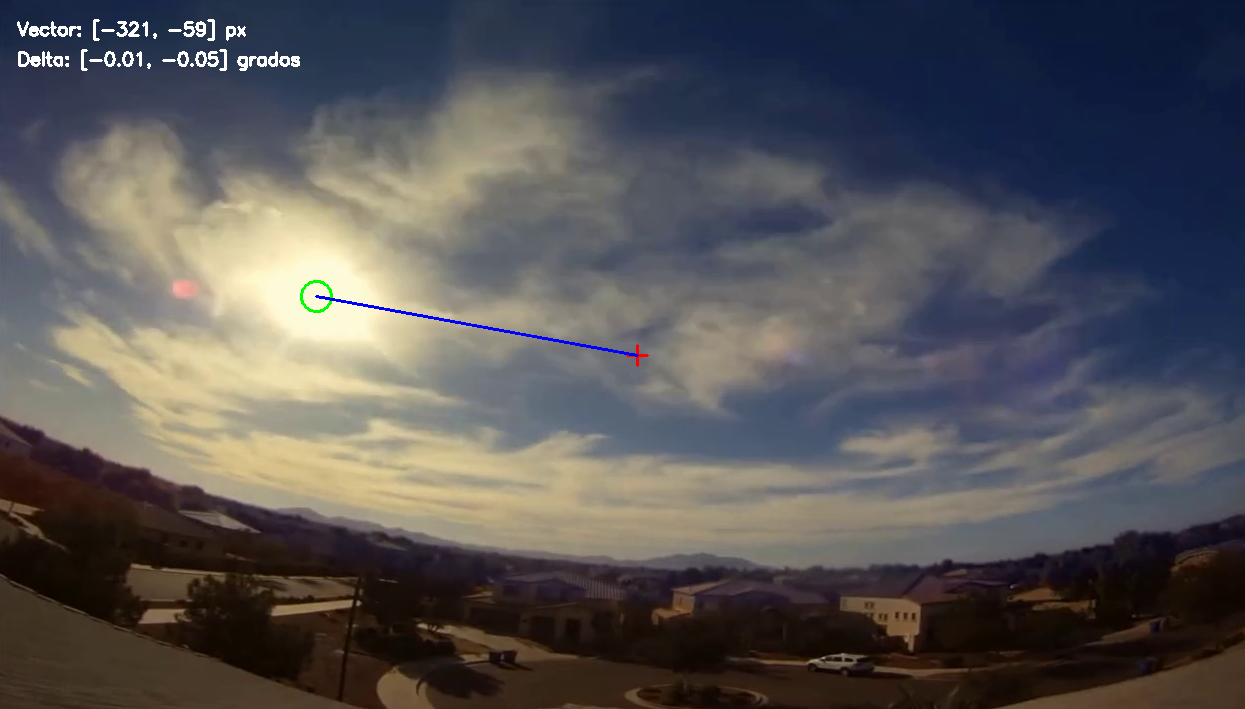
\includegraphics[width=\textwidth]{fig/deteccion_solar1}
        \caption{Frame original con datos superpuestos.}
        \label{fig:deteccion_solar1}
    \end{subfigure}
    \hfill % Espacio elástico para separar las imágenes
    % Segunda imagen
    \begin{subfigure}[b]{0.47\textwidth}
        \centering
        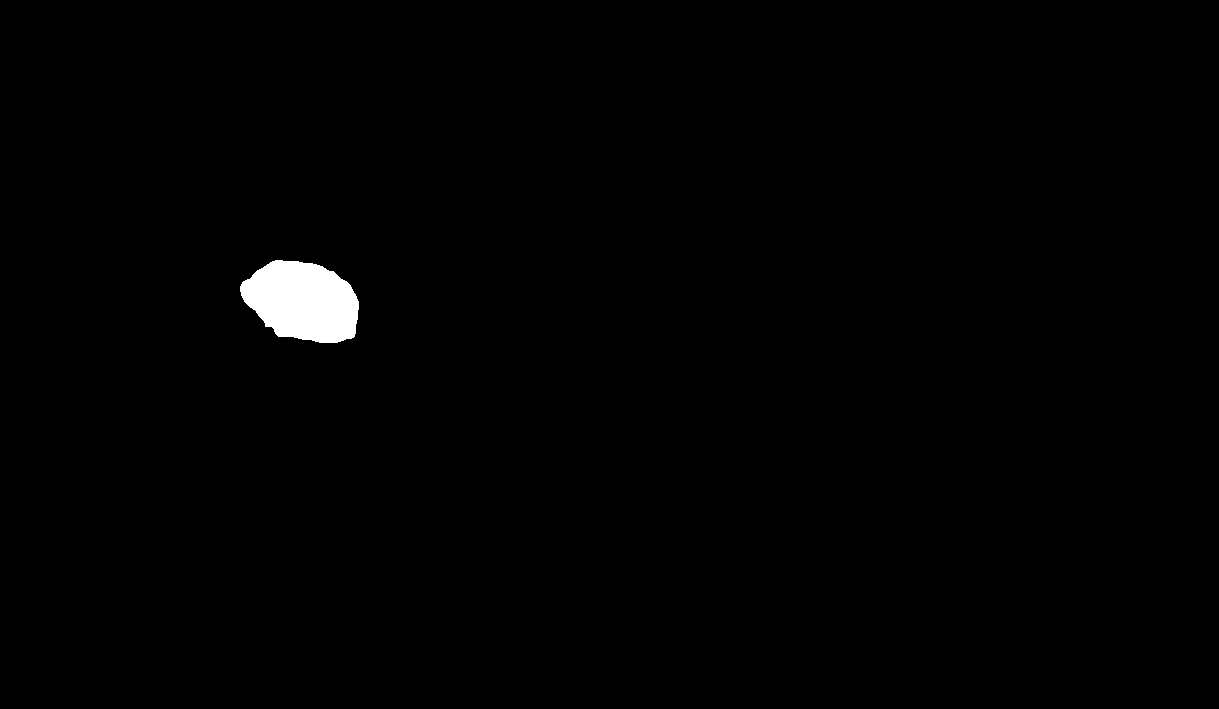
\includegraphics[width=\textwidth]{fig/deteccion_solar2}
        \caption{Frame binarizado resultante del procesado de imagen.}
        \label{fig:deteccion_solar2}
    \end{subfigure}
    
    \caption{Resultado del algoritmo de detección solar sobre vídeo real.}
    \label{fig:conjunto_deteccion}
\end{figure}

\subsection{Cinemática Inversa de la Plataforma Gough-Stewart}

Esta sección describe el desarrollo del modelo matemático de cinemática inversa implementado para gobernar los actuadores de la plataforma Gough-Stewart. Su función es, a partir de una orientación deseada expresada mediante los ángulos de Euler, determinar la longitud que debe adoptar cada actuador para alcanzar dicha posición. 

\subsubsection{Definición Geométrica del Sistema}\label{sec:Def_Geo}

La geometría del sistema se define mediante dos triángulos equiláteros concéntricos: la base fija y la plataforma móvil, cuyos vértices constituyen los puntos de anclaje de los seis actuadores lineales. Los vértices de ambas estructuras se generan distribuyendo tres puntos equiangularmente sobre una circunferencia de radio r. La base se centra en el origen $O=(0,0,0)$, el cálculo de la posición de los vertices se muestra en la ecuación \eqref{eq:PuntosBase}.

\begin{equation}
    \begin{gathered}
        B(\alpha) = r
        \begin{pmatrix}
            \cos(\alpha) \\
            \sin(\alpha) \\
            0
        \end{pmatrix}\\[6pt]
        \alpha_i = i \cdot \frac{2\pi}{3}, \quad i \in \{0,1,2\}
    \end{gathered}
    \label{eq:PuntosBase}
\end{equation}
Se define el punto $C$, el cual corresponde al punto focal de la lente. La plataforma móvil rota sobre este punto a una distancia constante $f=600mm$ igual a la distancia focal, con sus vértices desfasados angularmente respecto a los de la base para garantizar la no singularidad de la configuración inicial. Las coordenadas de los vertices siguen la expresión \eqref{eq:PuntosPlat}

\begin{equation}
    \begin{gathered}
        P(\beta) =
    		\begin{pmatrix}
		C_x \\
		C_y \\
		C_z
		\end{pmatrix}+r
        \begin{pmatrix}
            \cos(\beta) \\
            \sin(\beta) \\
            f
        \end{pmatrix}\\[6pt]
        \beta_i = i \cdot \frac{2\pi}{3}+\pi, \quad i \in \{0,1,2\}
    \end{gathered}
    \label{eq:PuntosPlat}
\end{equation}
Este desfase angular entre los vértices de la base y la plataforma es una característica intrínseca de la arquitectura Gough-Stewart, y su valor determina en gran medida el espacio de trabajo alcanzable por el mecanismo.

\subsubsection{Modelo Matemático de Cinemática Inversa}\label{sec:Cin_Inv}

El problema de cinemática inversa consiste en determinar las longitudes de los actuadores $l_i$ que producen una orientación deseada de la plataforma, definida por los ángulos de Euler $(\phi, \theta, \psi)$ correspondientes a las rotaciones en torno a los ejes $X,Y$ y $Z$ respectivamente.

\begin{enumerate}

	\item{Matrices de rotación elementales}
	
La orientación de la plataforma se describe mediante la composición de tres rotaciones elementales. La rotación en torno al eje $X$ de ángulo $\phi$ (cabeceo), la rotación en torno al eje $Y$ de ángulo $\theta$ (elevación) y la rotación en torno al eje $Z$ de ángulo $\psi$ (guiñada) se expresan en las ecuaciones \eqref{eq:RotCabeceo}, \eqref{eq:RotElev} y \eqref{eq:RotYaw} respectivamente.

\begin{equation}
R_x(\phi)=
\begin{pmatrix}
1 & 0 & 0 \\
0 & \cos\phi & -\sin\phi \\
0 & \sin\phi & \cos\phi
\end{pmatrix}
\label{eq:RotCabeceo}
\end{equation}



\begin{equation}
R_y(\theta)=
\begin{pmatrix}
\cos\theta & 0 & \sin\theta \\
0 & 1 & 0 \\
-\sin\theta & 0 & \cos\theta
\end{pmatrix}
\label{eq:RotElev}
\end{equation}

\begin{equation}
R_z(\psi)=
\begin{pmatrix}
\cos\psi & -\sin\psi & 0 \\
\sin\psi & \cos\psi & 0 \\
0 & 0 & 1
\end{pmatrix}
\label{eq:RotYaw}
\end{equation}

La orientación final de la plataforma se obtiene mediante la composición intrínseca $Z-Y-X$, que aplica primero la rotación en $Z$, luego en $Y$ y finalmente en $X$. Se muestra la expresión de la matriz de rotación combinada $R$ en la ecuación \eqref{eq:MatRot}.

\begin{equation}
R=R_z(\psi)\cdot R_y(\theta)\cdot R_x(\phi)
\label{eq:MatRot}
\end{equation}

	\item{Rotación de los vértices de la plataforma}

Cada vértice $p_i$ de la plataforma se rota respecto al punto focal $C$. Técnicamente, la rotación se aplica sobre el vector relativo definido entre el vértice y dicho punto, y el resultado se refiere nuevamente al sistema de coordenadas global. La ecuación \eqref{eq:VertRot} define esta transformación:

\begin{equation}
P^{rot}_i=R\cdot\left(P_i-C\right)+C
\label{eq:VertRot}
\end{equation}

Esta operación garantiza la invariancia de la posición del punto $C$ mientras rota los vértices de la plataforma móvil en torno a dicho punto. Este comportamiento es coherente con el modelo de control adoptado, puesto que permite modificar la orientación de la lente para el seguimiento solar manteniendo estático el punto focal, condición necesaria para la correcta concentración de la radiación sobre el lecho de sinterizado.

	\item{Cálculo de las longitudes de los actuadores}

Los seis actuadores lineales conectan cada vértice de la base $B$ con un vértice de la plataforma $P$, siguiendo el esquema de conexión cruzada propio de la arquitectura Gough-Stewart. La asignación de dichas conexiones se define mediante los índices detallados en \eqref{eq:Indices_conexion}:

\begin{equation}
\text{Plataforma: }[1,2,0,2,0,1],\quad\mathrm{Base:~}[0,0,1,1,2,2]
\label{eq:Indices_conexion}
\end{equation}

A partir de las coordenadas de los vértices de la base ($B_j$), la plataforma antes ($P_i$) y después de la rotación ($P_i^{rot}$), se determinan los vectores de los actuadores para ambas configuraciones, tal como se describe en \eqref{eq:calc_vec}:

\begin{equation}
\begin{aligned}
	\vec{l_i}=P_i-B_j\\
	\vec{l}_i^{rot}=P_i^{rot}-B_j
\end{aligned}
\label{eq:calc_vec}
\end{equation}
La magnitud escalar de cada actuador se obtiene mediante el cálculo del módulo de los vectores asociados, proceso ilustrado en la ecuación \eqref{eq:calc_mod}:

\begin{equation}
\begin{aligned}
	{l_i}=\|{\vec{l_i}}\|=\|P_i-B_j\|\\
	{l}_i^{rot}=\|{\vec{l}_i^{rot}}\|=\|P_i^{rot}-B_j\|
\end{aligned}
\label{eq:calc_mod}
\end{equation}

Finalmente, el desplazamiento lineal requerido para cada actuador se define como la diferencia de longitudes entre el estado rotado y el estado inicial:

\begin{equation}
\Delta l_i=l_i^{rot}-l_i
\label{eq:var_l}
\end{equation}

Un valor positivo en \eqref{eq:var_l} indica extensión del actuador; un valor negativo, contracción. Estos valores son la salida directa del modelo de cinemática inversa y constituyen las consignas enviadas a los actuadores físicos del sistema.

\subsubsection{Actualización Incremental del Estado}\label{sec:Act_Incr}

Un aspecto relevante de la implementación es que la posición de la plataforma se actualiza de forma incremental: al final de cada llamada a la función de cinemática inversa, la variable global \texttt{Ptri}, que almacena las coordenadas de los vértices de la plataforma antes de la rotación, se sobreescribe con la posición rotada \texttt{Ptrirot}. Esto significa que los ángulos ($\phi,\theta,\psi$) no se interpretan como orientaciones absolutas respecto a la posición de reposo original, sino como incrementos angulares aplicados sobre el estado inmediatamente anterior.

Este comportamiento es coherente con la salida del módulo de procesamiento de imagen descrito en \eqref{eq:CalcConversion}, donde $\Delta\theta$ y $\Delta\phi$ representan precisamente correcciones angulares incrementales calculadas a partir del error de apuntamiento instantáneo.

\subsubsection{Resumen del Flujo de Trabajo de Cinemática Inversa}

El proceso completo se resume en el diagrama de bloques de la Figura~\ref{fig:cin-inversa}, que muestra la secuencia de operaciones ejecutadas en cada llamada a la función de cinemática inversa. A partir de los incrementos angulares $(\Delta\phi,\Delta\theta,\Delta\psi)$ como entradas, el algoritmo construye la matriz de rotación combinada $\mathbf{R}$, aplica dicha rotación a los vértices de la plataforma respecto a su centro $C$, y calcula los vectores entre cada par de juntas base-plataforma para obtener las longitudes actuales de los seis actuadores. La variación respecto a la longitud de reposo, $\Delta l_i$, constituye la consigna enviada a cada actuador. La flecha de realimentación refleja la actualización incremental de \texttt{Ptri} descrita anteriormente.

\begin{figure}[htbp]
    \centering
    \begin{tikzpicture}[
        >=Triangle,
        node distance=0.5cm,
        io/.style={
            rectangle, draw=black!50, fill=black!8,
            rounded corners=4pt, minimum width=10cm,
            minimum height=0.9cm, font=\small, align=center
        },
        rot/.style={
            rectangle, draw=blue!50, fill=blue!12,
            rounded corners=4pt, minimum width=10cm,
            minimum height=1.4cm, font=\small, align=center
        },
        cin/.style={
            rectangle, draw=teal!60, fill=teal!12,
            rounded corners=4pt, minimum width=10cm,
            minimum height=1.4cm, font=\small, align=center
        },
        sal/.style={
            rectangle, draw=orange!70, fill=orange!18,
            rounded corners=4pt, minimum width=10cm,
            minimum height=0.9cm, font=\small, align=center
        },
        arrow/.style={->, thick, black!60}
    ]

    % 1. ENTRADAS
    \node[io] (entrada)
        {Entradas: $\Delta\phi,\;\Delta\theta,\;\Delta\psi$ \quad (ángulos de Euler)};

    % 2. MATRIZ DE ROTACIÓN
    \node[rot, below=of entrada] (rotmat)
        {Construcción de $\mathbf{R} = R_z \cdot R_y \cdot R_x$\\[4pt]
         \footnotesize $R_x(\phi)\; R_y(\theta)\; R_z(\psi)
         \;\rightarrow\; \mathbf{R} \in \mathrm{R}^{3\times3}$};

    % 3. ROTACIÓN PLATAFORMA
    \node[rot, below=of rotmat] (rotplat)
        {Rotación de la plataforma\\[4pt]
         \footnotesize $P'_i = \mathbf{R}\,(P_i - C) + C$
         \quad (rotar vértices respecto a $C$)};

    % 4. ÍNDICES
    \node[io, below=of rotplat] (indices)
        {Emparejamiento base $\leftrightarrow$ plataforma\\[3pt]
         \footnotesize
         \texttt{idx\_P} $= [1,2,0,2,0,1]$
         \qquad
         \texttt{idx\_B} $= [0,0,1,1,2,2]$};

    % 5. VECTORES ACTUADORES
    \node[cin, below=of indices] (vecact)
        {Vectores de actuadores\\[4pt]
         \footnotesize
         $\mathbf{a}_i = P'[\texttt{idx\_P}] - B[\texttt{idx\_B}]$
         \qquad
         $\mathbf{a}^0_i = P[\texttt{idx\_P}] - B[\texttt{idx\_B}]$};

    % 6. LONGITUDES
    \node[cin, below=of vecact] (long)
        {Longitudes de actuadores\\[4pt]
         \footnotesize
         $\|\mathbf{a}_i\|$ \; y \; $\|\mathbf{a}^0_i\|$
         \quad para $i = 1,\dots,6$};

    % 7. VARIACIÓN
    \node[sal, below=of long] (var)
        {Variación de cada actuador:\quad
         $\Delta l_i = \|\mathbf{a}_i\| - \|\mathbf{a}^0_i\|$};

    % 8. SALIDA
    \node[io, below=of var] (salida)
        {Salida: $\Delta l_1,\dots,\Delta l_6$
         \quad (consignas de extensión/contracción)};

    % ── FLECHAS PRINCIPALES ──
    \draw[arrow] (entrada)  -- (rotmat);
    \draw[arrow] (rotmat)   -- (rotplat);
    \draw[arrow] (rotplat)  -- (indices);
    \draw[arrow] (indices)  -- (vecact);
    \draw[arrow] (vecact)   -- (long);
    \draw[arrow] (long)     -- (var);
    \draw[arrow] (var)      -- (salida);

    % ── FLECHA DE REALIMENTACIÓN ──
    % Coordenadas auxiliares para los tres segmentos:
    %   salida.east → punto A (derecha) → punto B (misma Y que rotplat.east) → rotplat.east
    \coordinate (A) at ($(salida.east) + (2.8, 0)$);
    \coordinate (B) at ($(rotplat.east) + (2.8, 0)$);

    \draw[arrow, black!50]
        (salida.east) -- (A) -- (B) -- (rotplat.east);

    % Etiqueta a la derecha del segmento vertical, centrada entre A y B
    \node[font=\scriptsize, align=left, right=4pt]
        at ($(A)!0.5!(B)$)
        {\texttt{Ptri} $\leftarrow$ \texttt{Ptrirot}\\
         (actualización\\para siguiente\\iteración)};

    \end{tikzpicture}
    \caption{Diagrama de bloques del algoritmo de cinemática inversa.}
    \label{fig:cin-inversa}
\end{figure}

\end{enumerate}
\clearpage
\section{Cosimulación y Validación Virutal}
\label{sec:cosimulacion}

Esta sección describe la segunda fase del proceso metodológico: la validación cinemática del modelo mediante cosimulación entre el software de cálculo Python y el entorno \gls{CAD} de SolidWorks. El objetivo es doble: por un lado, verificar que el modelo matemático de cinemática inversa desarrollado en la sección anterior gobierna correctamente el gemelo digital del mecanismo; por otro, determinar el espacio de trabajo angular efectivo de la plataforma y contrastarlo con las trayectorias solares locales para las fechas astronómicas críticas, estableciendo así un criterio de viabilidad cuantitativo antes de proceder a la fabricación física.

\subsection{Arquitectura de la Cosimulación}

La cosimulación se articula mediante la biblioteca \texttt{win32com.client}, que expone la \gls{API} \gls{COM} de SolidWorks y permite controlar el ensamblaje CAD directamente desde Python en tiempo de ejecución. Esta aproximación elimina la necesidad de exportar resultados intermedios entre ambos entornos, estableciendo un canal de comunicación síncrono en el que Python actúa como controlador maestro y SolidWorks como motor de resolución geométrica y detección de colisiones.

La clase \texttt{SimuladorStewart} encapsula toda la lógica de la cosimulación y se estructura en torno a tres responsabilidades claramente diferenciadas: la definición geométrica del modelo, el cálculo de cinemática inversa y la interfaz con SolidWorks.

\subsection{Definición Geométrica del Modelo Real}

Esta fase se adapta el modelo geométrico general definido en la sección \ref{sec:Def_Geo}, dotando a los puntos de anclaje de la base ($B_i$) y la plataforma ($P_i$) de las coordenadas particulares de los cardanes correspondientes en el gemelo digital. Se definen entonces dos conjuntos de seis puntos cada uno así como también la coordenada particular del punto focal $C$ en el modelo, el cual constituye el centro de rotación de la plataforma móvil.

En SolidWorks, cada actuador está parametrizado mediante una cota de longitud denominada \texttt{D1@L}$i$, con un valor inicial de 200 mm, que se modifica en cada paso de la simulación para imponer el desplazamiento calculado por la cinemática inversa.

\subsection{Modelo de Cinemática Inversa con Coordenadas Reales}

El modelo de cinemática inversa implementado en esta fase sigue la misma formulación matricial descrita en la sección \ref{sec:Cin_Inv}, obteniendo el vector de cada anclaje de la plataforma relativo a $C$, aplicando la rotación deseada, devolviendo los vectores al sistema de referencia absoluto y obteniendo la longitud de los actuadores tras la  rotación como se describe en las ecuaciones desde \eqref{eq:VertRot} hasta \eqref{eq:var_l}.

Sin embargo, a diferencia del modelo de actualización descrito en \ref{eq:calc_mod}, la variación de cota que se inyecta en SolidWorks no es directamente $\Delta L_i$, sino que se adapta al sistema de referencia de la cota parametrizada del ensamblaje:

\begin{equation}
\delta_{cota,i}=\frac{\Delta L_i+L_{cota}^0}{1000}
\label{eq:delta_cota}
\end{equation}

donde $L_{cota}^0=200$ mm es el valor inicial de la cota en el modelo CAD y el factor $10^{-3}$ realiza la conversión de milímetros a metros, unidad requerida por la API de SolidWorks mediante el método \texttt{SetSystemValue3}.

\subsection{Interfaz con SolidWorks mediante la API COM}

La comunicación con SolidWorks se establece obteniendo una referencia al proceso activo mediante \texttt{GetActiveObject}, lo que requiere que la aplicación y el ensamblaje estén abiertos previamente. Una vez establecida la conexión, el ciclo de actualización del modelo sigue el siguiente procedimiento para cada paso de simulación:

En primer lugar, se activa el modo de escritura en base de datos con \texttt{SetAddToDB(True)}, que suspende la reconstrucción automática del ensamblaje y permite modificar todas las cotas de forma atómica antes de forzar una única reconstrucción. A continuación, se recupera cada parámetro por nombre mediante \texttt{model.Parameter(nombre\_cota)} y se actualiza su valor con \texttt{SetSystemValue3}. Finalmente, se desactiva el modo de escritura y se fuerza la reconstrucción del ensamblaje con \texttt{ForceRebuild3(False)}, momento en el que el motor geométrico de SolidWorks resuelve las relaciones de posición y actualiza la visualización del modelo.

\begin{figure}[htbp]
    \centering
    \begin{tikzpicture}[
        >=Triangle,
        node distance=0.5cm,
        io/.style={
            rectangle, draw=black!50, fill=black!8,
            rounded corners=4pt, minimum width=10cm,
            minimum height=0.9cm, font=\small, align=center
        },
        api/.style={
            rectangle, draw=blue!50, fill=blue!12,
            rounded corners=4pt, minimum width=10cm,
            minimum height=1.4cm, font=\small, align=center
        },
        geo/.style={
            rectangle, draw=teal!60, fill=teal!12,
            rounded corners=4pt, minimum width=10cm,
            minimum height=0.9cm, font=\small, align=center
        },
        sal/.style={
            rectangle, draw=orange!70, fill=orange!18,
            rounded corners=4pt, minimum width=10cm,
            minimum height=0.9cm, font=\small, align=center
        },
        arrow/.style={->, thick, black!60}
    ]

    % 1. ENTRADA
    \node[io] (entrada)
        {Entrada: $\Delta l_1,\dots,\Delta l_6$ \quad
         (longitudes de actuadores calculadas)};

    % 2. ACTIVAR MODO ESCRITURA
    \node[api, below=of entrada] (setdb)
        {\texttt{SetAddToDB(True)}\\[4pt]
         \footnotesize
         Suspende la reconstrucción automática del ensamblaje.
         Las cotas se modifican de forma atómica.};

    % 3. BUCLE ACTUALIZACIÓN DE COTAS
    \node[api, below=of setdb, minimum height=1.8cm] (cotas)
        {Actualización de cotas \quad
         \texttt{for} $i = 1,\dots,6$\\[4pt]
         \footnotesize
         \texttt{model.Parameter(nombre\_cota $_i$)}
         $\;\rightarrow\;$
         \texttt{SetSystemValue3($\Delta l_i$)}};

    % 4. DESACTIVAR MODO ESCRITURA
    \node[api, below=of cotas] (unsetdb)
        {\texttt{SetAddToDB(False)}\\[4pt]
         \footnotesize
         Cierra el bloque de escritura atómica.
         El ensamblaje aún no ha sido reconstruido.};

    % 5. FORZAR RECONSTRUCCIÓN
    \node[geo, below=of unsetdb] (rebuild)
        {\texttt{ForceRebuild3(False)} \quad
         El motor geométrico de SolidWorks resuelve
         las relaciones de posición.};

    % 6. ACTUALIZACIÓN VISUAL
    \node[sal, below=of rebuild] (visual)
        {Actualización de la visualización del modelo 3D en SolidWorks};

    % ── FLECHAS ──
    \draw[arrow] (entrada)  -- (setdb);
    \draw[arrow] (setdb)    -- (cotas);
    \draw[arrow] (cotas)    -- (unsetdb);
    \draw[arrow] (unsetdb)  -- (rebuild);
    \draw[arrow] (rebuild)  -- (visual);

   % ── RECTÁNGULO: bloque atómico ──
    \node[
        draw=black!40,
        dashed,
        thick,
        rounded corners=6pt,
        inner sep=8pt,
        fit=(setdb)(cotas)(unsetdb),
        label={[font=\scriptsize, black!50]right:Bloque atómico}
    ] {};

    \end{tikzpicture}
    \caption{Diagrama de bloques del proceso de inyección de datos en la
    API de SolidWorks.}
    \label{fig:inyeccion-solidworks}
\end{figure}

\subsection{Mapeado del Espacio de Trabajo Angular}

El método principal de validación consiste en un barrido sistemático del espacio angular $(\phi, \theta)$ con una resolución de $5^{\circ}$ en ambos ejes, cubriendo el rango $[-30^{\circ},30^{\circ}]$ en cada dirección. Para cada punto del barrido se ejecuta el siguiente procedimiento de clasificación, que asigna uno de tres estados posibles:

\begin{itemize}

	\item {Estado 0 – Fuera de carrera:} las longitudes calculadas por la cinemática inversa exceden los límites físicos de los actuadores
	
	\item{Estado 1 – Error CAD: las longitudes son geométricamente admisibles pero el ensamblaje no puede resolver sus relaciones de posición tras la doble reconstrucción forzada, indicando una colisión entre componentes o una singularidad cinemática no detectada analíticamente.}
	
	\item{Estado 2 – Posición válida: los actuadores están dentro de rango y el ensamblaje resuelve correctamente todas sus relaciones de posición.}
	
\end{itemize}

Cada combinación de ángulos se mapea con un punto verde si es una posición válida y con una cruz roja si le corresponde el estado 0 o 1. Como resultado se obtiene un gráfico discretizado de combinaciones angulares válidas y no válidas obteniendo así el espacio de trabajo efectivo de la plataforma de Gough-Stewart para la rotación sobre el punto focal $C$.

\subsection{Superposición con Trayectorias Solares}

Los resultados del mapeado se superponen con las trayectorias solares calculadas analíticamente para la latitud de la ubicación de instalación en Toledo ($\varphi=39.866^{\circ} N$), correspondiente a tres fechas astronómicas de referencia: el solsticio de verano (día 172), el equinoccio (día 81) y el solsticio de invierno (día 355).

Para cada fecha, la declinación solar se calcula mediante la ecuación de Cooper:

\begin{equation}
	\delta=23{,}44^{\circ}\cdot \sin{\left(\frac{360}{365}(d-81)\right)}
	\label{eq:eqCooper}
\end{equation}

Donde $23{,}44^{\circ}$ es la inclinación del eje de rotación respecto el plano de la eclíptica; $d$ es el dia del año al que se le aplica un desfase de 81 dias de forma que en el equinoccio la declinación sea nula.

El ángulo cenital $\theta_z$ y el ángulo acimutal $\phi_a$ se obtienen a partir de las ecuaciones de posición solar estándar en función del ángulo horario $\omega$:

\begin{equation}
    \begin{aligned}
        \cos\theta_z &= \sin\delta\sin\varphi+\cos\delta\cos\varphi\cos\omega \\[1ex]
        \cos\phi_a &= \frac{\sin\delta-\cos\theta_z\sin\varphi}{\sin\theta_z\cos\varphi}
    \end{aligned}
    \label{eq:angulos_solares}
\end{equation}

Debe tenerse en cuenta que las ecuaciones \eqref{eq:angulos_solares} emplean el convenio astronómico estándar: el ángulo cenital $\theta_z$ se mide desde la vertical del observador (cenit), siendo nulo cuando el sol se encuentra directamente sobre este, y el ángulo acimutal $\phi_a$ se mide desde el sur geográfico, tomando valor nulo en el mediodía solar, momento en que el ángulo horario $\omega=0$.

En la Figura \ref{fig:RutasSolares} se representan la variación del ángulo cenital $\theta_z$ y del ángulo acimutal $\phi_a$ en función de las horas transcurridas desde el mediodía solar, para las tres fechas astronómicas de referencia. La gráfica inferior muestra la trayectoria solar resultante en el plano acimutal-cenital, donde el eje vertical, invertido, representa el ángulo cenital creciente desde el cenit hacia el horizonte. Puede observarse cómo el solsticio de verano produce la trayectoria de mayor elevación y amplitud acimutal, mientras que el solsticio de invierno queda significativamente más próximo al horizonte y restringido a un rango acimutal más estrecho.

\begin{figure}[H]
	\centering
		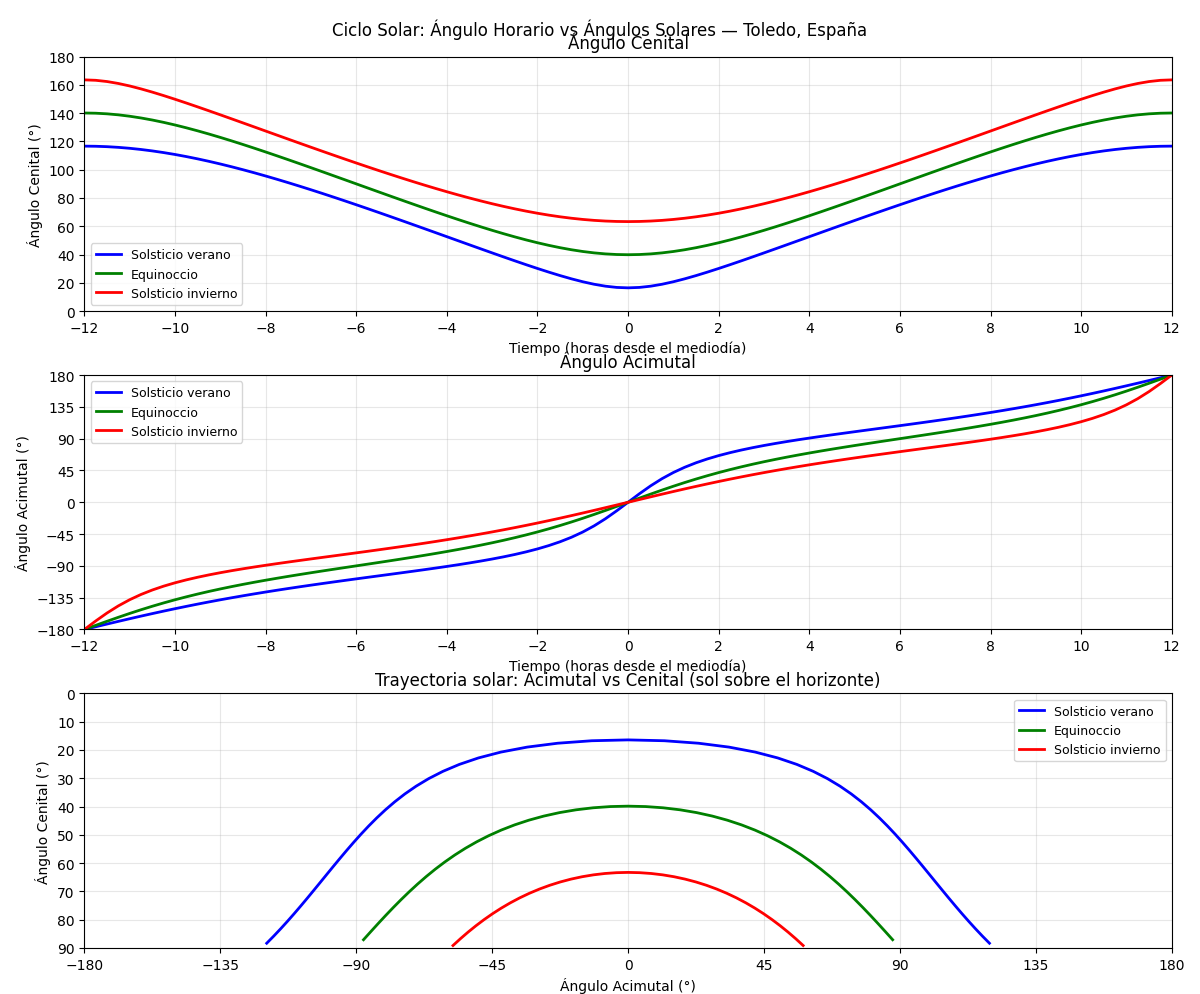
\includegraphics[width=0.8\textwidth]{fig/Rutas_Solares}
        \caption{Ciclo solar para Toledo, España ($\varphi = 39{,}87^{\circ}N$): variación del ángulo cenital $\theta_z$ (superior) y acimutal $\phi_a$ (centro) en función de las horas desde el mediodía solar, y trayectoria resultante en el plano $\phi_a$-$\theta_z$ con el sol sobre el horizonte (inferior), para el solsticio de verano, el equinoccio y el solsticio de invierno.}
        \label{fig:RutasSolares}
\end{figure}

Una vez calculadas las rutas solares, las superponemos en el plano $\phi_a$-$\theta_z$ junto con el mapa de puntos del mapeado de espacio de trabajo. En la figura \ref{fig:EspacioTrabajo} se muestran los resultados.

\begin{figure}[H]
	\centering
		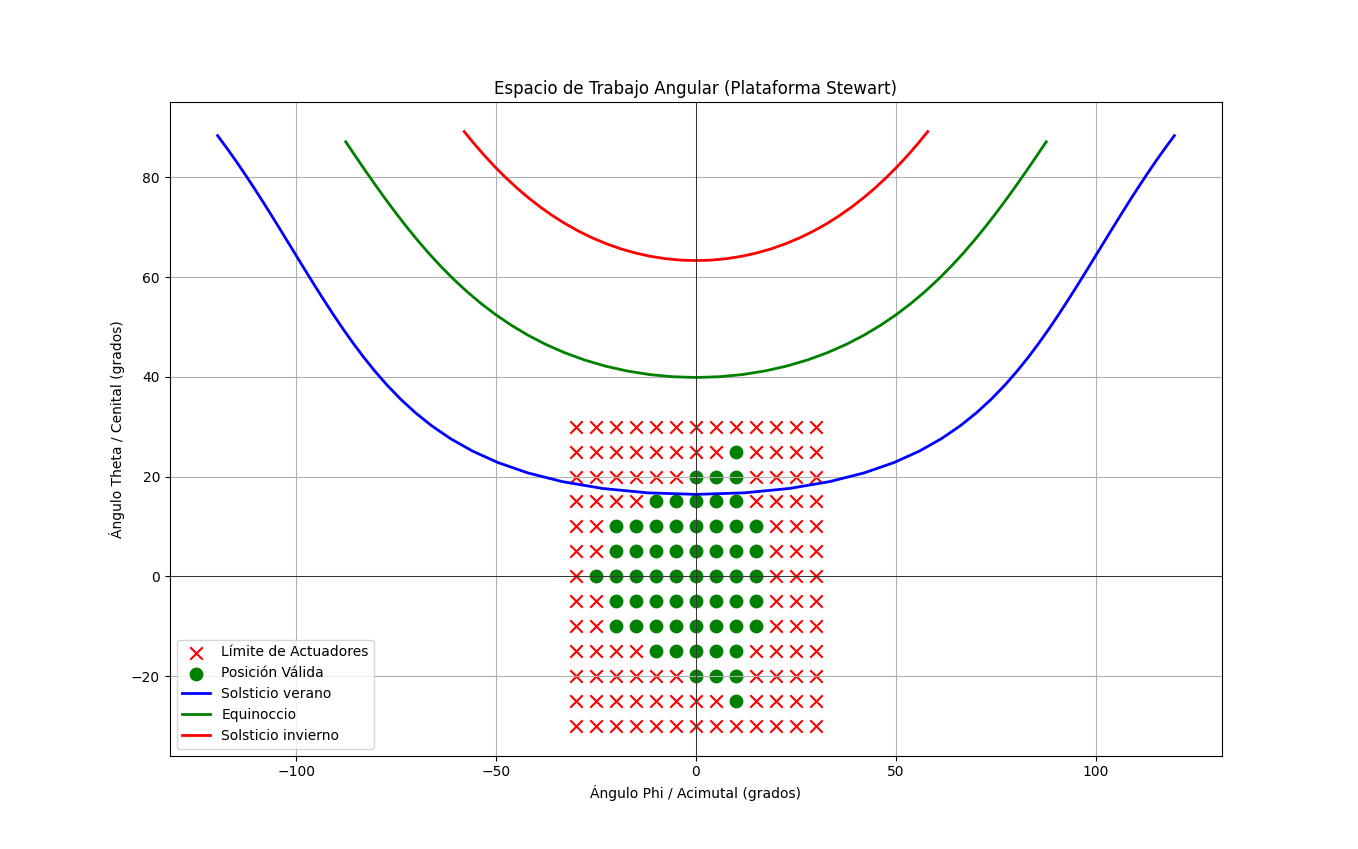
\includegraphics[width=1\textwidth]{fig/Espacio_Trabajo_Stewart}
        \caption{Resultado del mapeado del espacio de trabajo angular de la plataforma Gough-Stewart superpuesto con las trayectorias solares calculadas para Toledo.}
        \label{fig:EspacioTrabajo}
\end{figure}

Los puntos del barrido clasificados como posición válida (círculos verdes) forman una región compacta centrada en el origen, abarcando aproximadamente $\pm 20^{\circ}$ en $\theta$ y $\pm 25^{\circ}$ en $\phi$.

La conclusión más relevante que se extrae de la figura es que ninguna de las tres trayectorias solares queda contenida dentro del espacio de trabajo durante un intervalo de tiempo aprovechable. Las curvas del equinoccio (verde) y del solsticio de invierno (rojo) discurren en la región superior de la gráfica, muy por encima de los $25^{\circ}$ de ángulo cenital máximo alcanzable por la plataforma. Por su parte, la curva del solsticio de verano (azul) alcanza un ángulo cenital mínimo de $16^{\circ}$ durante el mediodía solar; sin embargo, como se aprecia en la Figura \ref{fig:RutasSolares}, el intervalo en el que la trayectoria permanece dentro del espacio de trabajo no supera la hora, lo que hace inviable cualquier aprovechamiento energético útil incluso en el día de mayor irradiación del año.

Esta incompatibilidad entre el espacio de trabajo del mecanismo y las exigencias angulares del ciclo solar constituye el criterio de descarte de la arquitectura Gough-Stewart clásica en la metodología del proyecto, justificando el rediseño iterativo descrito en la sección \ref{sec:Metodologia}.

\section{Síntesis de la Arquitectura Alternativa}

\subsection{Planteamiento del rediseño}
La incompatibilidad cinemática entre el espacio de trabajo de la plataforma Gough-Stewart y los requerimientos de seguimiento solar, expuesta en la Sección \ref{sec:Metodologia}, motiva un rediseño completo de la arquitectura mecánica. En coordinación con el director del proyecto, Antonio González Rodríguez, se propone abandonar la topología paralela espacial en favor de una arquitectura híbrida formada por dos mecanismos planos de lazo cerrado cinemáticamente desacoplados, uno por cada eje de orientación. Este conjunto se compone de:

\begin{description}
    \item[Mecanismo acimutal:] Una cadena plana de seis barras tipo Stephenson III, accionada por un único actuador lineal y dispuesta sobre el bastidor fijo. Gobierna el giro de la plataforma móvil alrededor del eje vertical.
    \item[Mecanismo cenital:] Un mecanismo plano de biela-manivela montado sobre el eslabón de salida del mecanismo acimutal. Gobierna la rotación de la estructura portadora de la lente de Fresnel alrededor de un eje horizontal solidario al subconjunto acimutal.
\end{description}

El desacoplamiento cinemático entre ambos mecanismos constituye la propiedad distintiva de la arquitectura: el accionamiento del actuador acimutal no produce variación alguna en el ángulo cenital, y viceversa. Esta independencia simplifica el modelo cinemático del conjunto a la composición trivial de dos problemas planos resolubles por separado, evitando los acoplamientos cruzados característicos de las plataformas paralelas espaciales y permitiendo gobernar cada eje de forma independiente.

\subsection{Mecanismo acimutal: cadena Stephenson tipo III}

\subsubsection{Definición geométrica}
\label{sec:def_geo_acimut}
El mecanismo acimutal sigue el esquema mostrado en la figura \ref{fig:esquema_acimut}. Se trata de una cadena cinemática plana de seis eslabones que constituye una variante de la topología Stephenson tipo III, caracterizada por la presencia de un eslabón ternario que comparte dos pares cinemáticos con sendos lazos cerrados. La identificación y función de cada componente es la siguiente:

\begin{description}
	\item[Carro $A_2$ (actuador lineal):] Carro deslizante que se desplaza a lo largo de la guía horizontal del actuador lineal, con una carrera útil de 300~mm entre las posiciones extremas $A_3$ (carrera nula, $s=0$) y $A_1$ (carrera máxima, $s=300$~mm).
	
	\item[Barra 3 (biela de entrada):] Barra rígida que conecta el carro del actuador (punto $A_2$) con el extremo $B$ del eslabón ternario.
	
	\item[Eslabón 4 (ternario):] Eslabón rígido en forma de triángulo $OBC$ que pivota alrededor del punto fijo $O$. Sus tres vértices articulan, respectivamente, con el bastidor en $O$, con la biela 3 en $B$ y con la biela 5 en $C$.
	
	\item[Barra 5 (biela de acoplamiento):] Barra rígida que transmite el movimiento desde el vértice $C$ del ternario hasta el vértice $D$ del eslabón de salida.
	
	\item[Barra 6 (barra de salida):] Barra rígida que pivota alrededor del punto fijo $Q$ y constituye la salida del mecanismo. Su orientación angular respecto a la horizontal, denotada $\phi$, es el ángulo acimutal de la plataforma móvil. Sobre este eslabón se monta el mecanismo cenital descrito en la Sección \ref{sec:Mec_Cenital}.
\end{description}


\begin{figure}[h!]
	\centering
	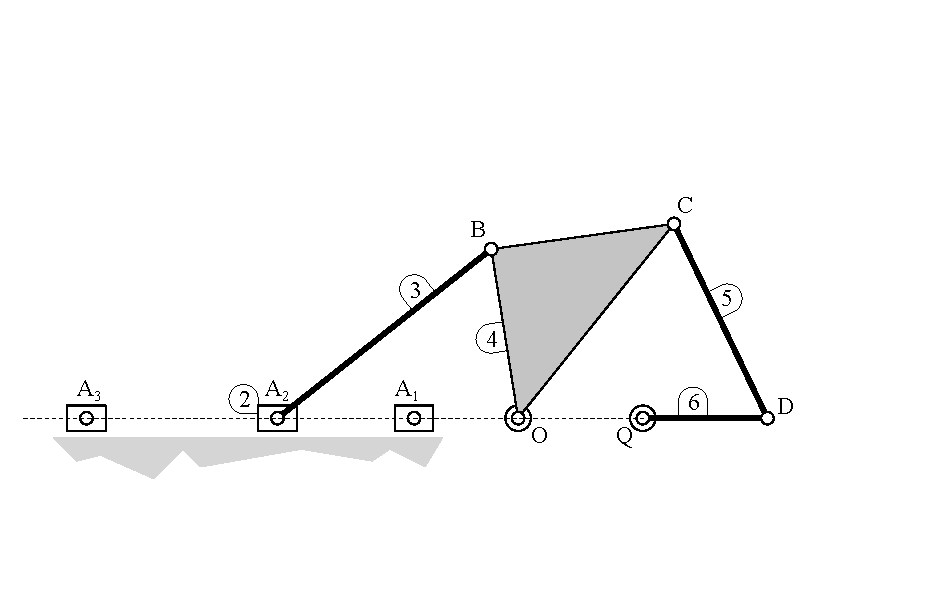
\includegraphics[width=0.9\textwidth]{fig/esquema_acimut}
	\caption{Esquema del mecanismo acimutal de seis barras tipo Stephenson III. El sur está hacia la derecha dirección QD. El dibujo representa la posición del mecanismo en el medio día.}
	\label{fig:esquema_acimut}
\end{figure}

Las dimensiones nominales adoptadas para el dimensionamiento del mecanismo se recogen en la Tabla~\ref{tab:dim_stephenson}.

\begin{table}[H]
    \centering
    \begin{tabular}{lll}
        \toprule
        \textbf{Parámetro} & \textbf{Símbolo} & \textbf{Valor [mm]} \\
        \midrule
        Longitud de la barra 3 ($A_2 B$)       & $\rho_3$  & $262{,}57$ \\
        Cara $OB$ del ternario                 & $OB$      & $165{,}01$ \\
        Cara $OC$ del ternario                 & $OC$      & $240{,}00$ \\
        Cara $BC$ del ternario                 & $BC$      & $177{,}53$ \\
        Longitud de la barra 5 ($CD$)          & $\rho_5$  & $120\sqrt{3}\;\approx\;207{,}85$ \\
        Longitud de la barra de salida ($QD$)  & $\rho_6$  & $120{,}00$ \\
        Distancia entre pivotes fijos          & $OQ$      & $120{,}00$ \\
        Distancia $OA_3$ (carrera nula)        & $OA_{3}$  & $422{,}43$ \\
        \bottomrule
    \end{tabular}
    \caption{Dimensiones nominales del mecanismo acimutal Stephenson III. El ángulo interior 
    fijo del eslabón ternario en el vértice $O$ vale $\angle BOC = 47{,}7^{\circ}$.}
    \label{tab:dim_stephenson}
\end{table}

El sistema de coordenadas adoptado para el análisis tiene su origen en el pivote $O$, con el eje $X$ horizontal apuntando hacia el pivote $Q$ (esto es, $Q=(OQ,\,0)$) y el eje $Y$ orientado positivamente hacia el semiplano donde se encuentra el ternario.

\subsubsection{Cinemática directa}
\label{sec:cinematica_acimut}
La cinemática directa del mecanismo consiste en determinar el ángulo de salida $\phi$ (orientación de la barra 6) a partir de la carrera $s$ del actuador. El problema admite una resolución analítica completa mediante la descomposición de la cadena en dos lazos geométricos consecutivos, encadenados a través del eslabón ternario.

\begin{description}
\item [Lazo 1: triángulo $OA_2B$.]
Conocida la carrera del actuador $s$, la distancia entre el pivote $O$ y el carro $A_2$ es:

\begin{equation}
    OA = OA_3 - s= 422,4261 - s
    \label{eq:OA_acimutal}
\end{equation}

El triángulo $OA_2B$ queda definido por los tres lados $OA$, $OB$ y $\rho_3$. Aplicando 
la ley del coseno en el vértice $O$ se obtiene el ángulo interior entre $OA_2$ y $OB$:

\begin{equation}
    \angle BOA_2 = \arccos\!\left( \frac{OA^2 + OB^2 - \rho_3^2}{2 \cdot OA \cdot OB} \right)
    \label{eq:angBOA2}
\end{equation}

Dado que el carro $A_2$ se encuentra sobre el semieje $X$ negativo respecto a $O$, el ángulo del segmento $OB$ medido desde el semieje $X$ positivo resulta:

\begin{equation}
    \theta_{OB} = \pi - \angle BOA_2
    \label{eq:thetaOB}
\end{equation}

\item[Eslabón ternario.]
La rigidez del eslabón 4 impone una relación geométrica fija entre las direcciones $OB$ y $OC$: el ángulo interior del ternario en el vértice $O$ tiene un valor de $\angle BOC = 47{,}7^{\circ}$, medido en sentido horario desde $OB$ hacia $OC$. Por tanto:

\begin{equation}
    \theta_{OC} = \theta_{OB} -\frac{2\pi}{360^{\circ}}\cdot 47{,}7^{\circ}
    \label{eq:thetaOC}
\end{equation}

Las coordenadas del vértice $C$ en el sistema centrado en $O$ se obtienen directamente:

\begin{equation}
    \begin{aligned}
        C_x &= OC \cdot \cos(\theta_{OC}) \\
        C_y &= OC \cdot \sin(\theta_{OC})
    \end{aligned}
    \label{eq:coordC}
\end{equation}

\item[Lazo 2: triángulo $QCD$.]
Conocidas las coordenadas de $C$ y la posición fija de $Q=(OQ,\,0)$, se calcula la distancia entre ambos puntos y la orientación del segmento $QC$ respecto a la horizontal:

\begin{equation}
    \begin{aligned}
        d_{QC}   &= \sqrt{(C_x - Q_x)^2 + (C_y - Q_y)^2} \\
        \alpha_{QC} &= \arctan\frac{C_y - Q_y}{C_x - Q_x}
    \end{aligned}
    \label{eq:QC}
\end{equation}

El triángulo $QCD$ tiene lados $\rho_6$ (barra de salida $QD$), $d_{QC}$ y $\rho_5$ (biela de acoplamiento $CD$). Aplicando nuevamente la ley del coseno en el vértice $Q$ se obtiene el ángulo interior entre $QC$ y $QD$:

\begin{equation}
    \angle CQD = \arccos\!\left( \frac{\rho_6^2 + d_{QC}^2 - \rho_5^2}{2 \cdot \rho_6 \cdot d_{QC}} \right)
    \label{eq:angCQD}
\end{equation}

El ángulo de salida $\phi$ (orientación de la barra 6 respecto a la horizontal) resulta:

\begin{equation}
    \phi(s) = \alpha_{QC} - \angle CQD
    \label{eq:phi_directa}
\end{equation}

La concatenación de las ecuaciones \eqref{eq:OA_acimutal}--\eqref{eq:phi_directa} constituye el modelo de cinemática directa $\phi = f(s)$. La figura~\ref{fig:curva_phi_s} representa la curva resultante para todo el barrido del actuador, $s \in [0,\,300]$~mm. Puede observarse que la función es estrictamente monótona en el rango operativo, lo que garantiza la unicidad de la solución inversa. La línea discontinua roja indica la posición de mediodía solar ($\phi = 0^{\circ}$), correspondiente a $s \approx 189{,}70$~mm. El barrido angular total cubre 240$^{\circ}$.

\begin{figure}[htbp]
    \centering
    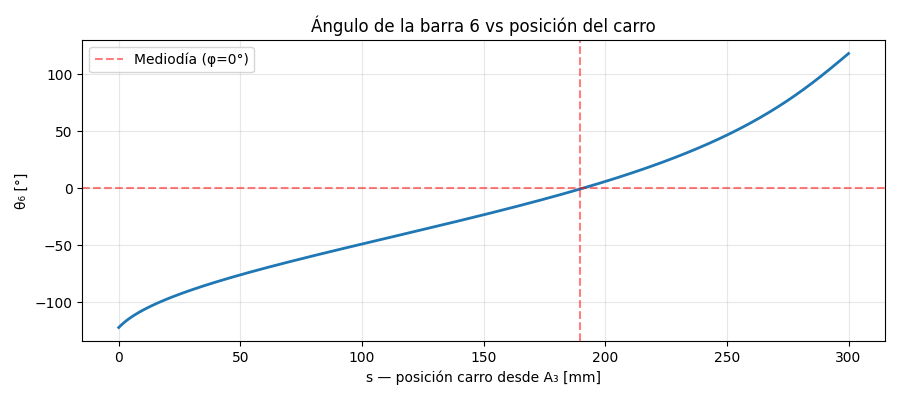
\includegraphics[width=0.85\textwidth]{fig/curva_phi_s}
    \caption{Curva de cinemática directa del mecanismo acimutal: ángulo de salida $\phi$ de la barra 6 en función de la carrera $s$ del actuador. }
    \label{fig:curva_phi_s}
\end{figure}

\end{description}

\subsection{Mecanismo cenital: biela-manivela}
\label{sec:Mec_Cenital}

El segundo elemento de la arquitectura robótica es un mecanismo plano biela-manivela montado solidariamente sobre la barra de salida del mecanismo acimutal (eslabón~6, Figura~\ref{fig:esquema_acimut}). Su función es gobernar la inclinación de la estructura portadora de la lente de Fresnel respecto al plano horizontal local del subconjunto acimutal, ofreciendo el segundo grado de libertad necesario para el seguimiento solar.

\subsubsection{Definición geométrica}
El mecanismo cenital sigue el esquema mostrado en la Figura~\ref{fig:esquema_cenital}. Se compone de cinco eslabones articulados formando un lazo plano cerrado característico de la cadena cinemática biela-manivela. Su disposición es vertical: la columna estructural se eleva desde un pivote anclado al punto rotativo Q del mecanismo acimutal descrito en \ref{sec:def_geo_acimut} (en \ref{fig:esquema_cenital} referido como $O$) hasta el pivote $O'$ del portalente, sobre el cual se monta la lente de Fresnel.

\begin{description}
	\item[Eslabón 1 (biela):] barra rígida que conecta el carro del actuador con el vértice izquierdo del portalente, transmitiendo la fuerza axial del actuador como par de rotación sobre el pivote $O'$.
	
	\item[Eslabones 2 y 3 (portalente):] los dos lados del eslabón ternario que pivota alrededor de $O'$. El portalente es la pieza solidaria a la lente de Fresnel, y su orientación angular respecto al bastidor vertical constituye el ángulo de salida $\theta$ del mecanismo.
	
	\item[Eslabón 4 (bastidor vertical):] columna estructural que conecta los dos pivotes fijos $O$ y $O'$. Define la referencia angular desde la cual se mide el ángulo de salida.
	
	\item[Eslabón 5 (referencia horizontal):] distancia fija entre el actuador lineal A y la barra $rho_4$.
	
	\item[Carro del actuador:] elemento deslizante que se desplaza a lo largo de una guía rectilínea paralela al eslabón 4, con una carrera útil de 300~mm entre las posiciones extremas $A_1$ (carrera nula, $A=0$) y $A_2$ (carrera máxima, $A=300$~mm).
\end{description}

\begin{figure}[htbp]
    \centering
    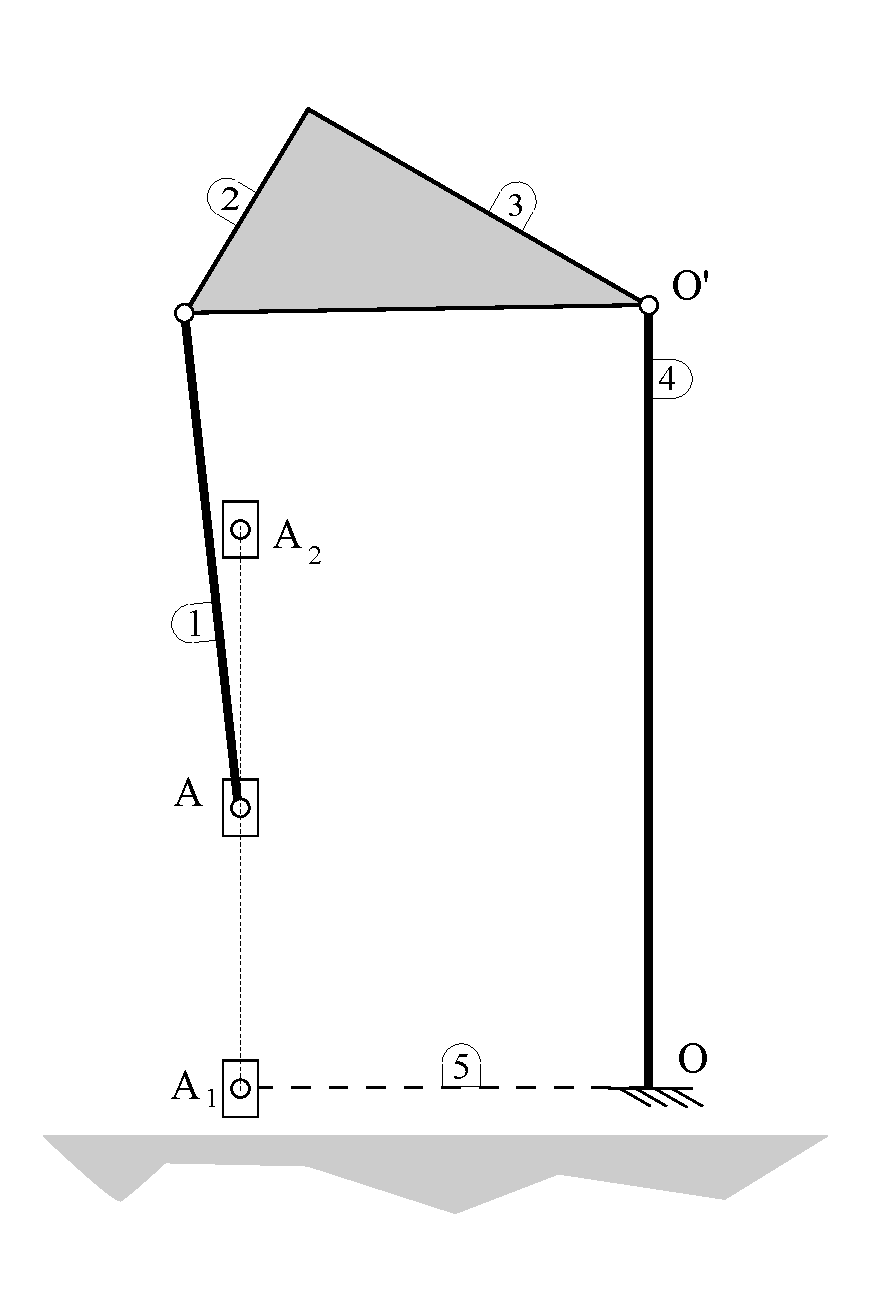
\includegraphics[width=0.5\textwidth]{fig/esquema_cenital}
	\caption{Esquema del mecanismo cenital.}
	\label{fig:esquema_cenital}
\end{figure}

Las dimensiones nominales del mecanismo se recogen en la Tabla~\ref{tab:dim_cenital}.

\begin{table}[htbp]
    \centering
    \begin{tabular}{lll}
        \toprule
        \textbf{Parámetro} & \textbf{Símbolo} & \textbf{Valor [mm]} \\
        \midrule
        Longitud de la biela (eslabón~1)              & $\rho_1$ & $316{,}57$ \\
        Longitud del eslabón~2 del portalente         & $\rho_2$ & $120{,}00$ \\
        Longitud del eslabón~3 del portalente         & $\rho_3$ & $200{,}00$ \\
        Longitud del bastidor vertical (eslabón 4)        & $\rho_4$ & $400{,}00$ \\
        Offset perpendicular guía--$\rho_4$               & $\rho_5$ & $221{,}08$ \\
        \bottomrule
    \end{tabular}
    \caption{Dimensiones nominales del mecanismo cenital biela-manivela. La unión empotrada entre los eslabones~2 y~3 mantiene constante un ángulo recto en el apex superior del portalente.}
    \label{tab:dim_cenital}
\end{table}

\subsubsection{Cinemática directa}
\label{sec:cin_dir_cenit}
La cinemática directa determina el ángulo cenital $\theta$ del portalente a partir de la carrera $A$ del actuador. La estrategia adoptada descompone el lazo cinemático en dos triángulos rectángulos auxiliares cuyas hipotenusas constituyen los lados móviles de un triángulo de cierre con la biela $\rho_1$.

\begin{description}
\item[Triángulo del lado del portalente.]
Los segmentos $\rho_2$ y $\rho_3$ definen un triángulo rectángulo cuya hipotenusa $b$ es la distancia del extremo superior de $\rho_4$ al punto de anclaje de la biela sobre el portalente. Esta distancia es constante dado que ambos segmentos son solidarios al eslabón rotativo:

\begin{equation}
    b = \sqrt{\rho_2^{2} + \rho_3^{2}}
    \label{eq:b_cenital}
\end{equation}

El ángulo interior de dicho triángulo en el vértice $O'$, denotado $\theta_{B}$, es asimismo constante y vale:

\begin{equation}
    \theta_{B} = \arctan\!\left( \frac{\rho_2}{\rho_3} \right)
    \label{eq:thetaB_cenital}
\end{equation}

\item[Triángulo del lado del actuador.]
Los segmentos $\rho_5$ y $(\rho_4 - A)$ definen un triángulo rectángulo cuya hipotenusa $a$ es la distancia desde la posición del actuador lineal hasta $O'$. A diferencia del 
caso anterior, esta longitud depende de la carrera del actuador:

\begin{equation}
    a(A) = \sqrt{\rho_5^{2} + (\rho_4 - A)^{2}}
    \label{eq:a_cenital}
\end{equation}

El ángulo interior de este triángulo, denotado $\theta_{A}$, también depende de la carrera:

\begin{equation}
    \theta_{A}(A) = \arctan\!\left( \frac{\rho_5}{\rho_4 - A} \right)
    \label{eq:thetaA_cenital}
\end{equation}

\item[Triángulo de cierre.]
Las hipotenusas $a$ y $b$ confluyen en un vértice común y se unen, en sus extremos opuestos, mediante el acoplador $\rho_1$. Estos tres segmentos forman el triángulo de cierre del lazo cinemático. Aplicando el teorema del coseno se obtiene el ángulo interior $\theta_{C}$ entre las hipotenusas:

\begin{equation}
    \theta_{C}(A) = \arccos\!\left( \frac{a^{2} + b^{2} - \rho_1^{2}}{2 \cdot a \cdot b} \right)
    \label{eq:thetaC_cenital}
\end{equation}

\item[Ángulo de salida.]
El ángulo cenital $\theta$ del portalente se obtiene como el resto de $\pi$ menos la suma algebraica de los tres ángulos parciales anteriores, completando el lazo:

\begin{equation}
    \theta(A) = \pi - \theta_{A}(A) - \theta_{B} - \theta_{C}(A)
    \label{eq:theta_directa}
\end{equation}

La concatenación de las ecuaciones \eqref{eq:b_cenital}--\eqref{eq:theta_directa} constituye el modelo de cinemática directa $\theta = g(A)$ del mecanismo cenital. La Figura~\ref{fig:curva_theta_A} representa la curva resultante para todo el barrido del actuador. Análogamente al caso acimutal, la función es estrictamente monótona en el rango operativo, garantizando la unicidad de la solución inversa. El barrido angular total cubre los 80$^{\circ}$ comprendidos entre la posición horizontal (sol cerca del horizonte) y la vertical (sol en el cenit), abarcando el intervalo de horas solares de mayor irradiancia útil.

\begin{figure}[htbp]
    \centering
    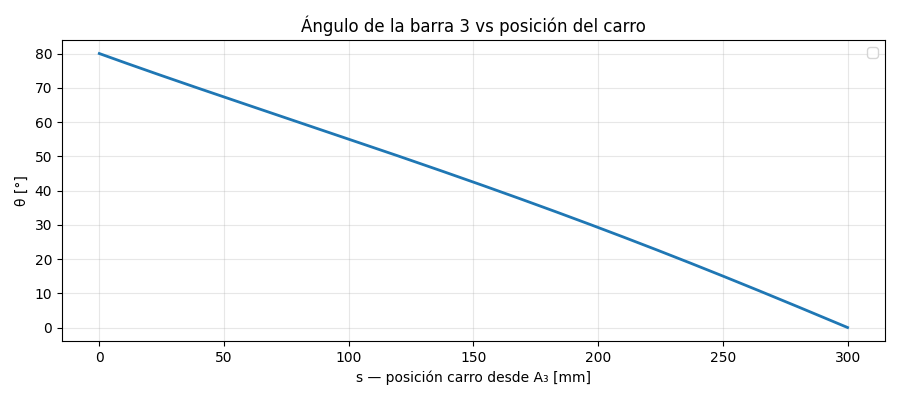
\includegraphics[width=0.85\textwidth]{fig/curva_theta_A}
    \caption{Curva de cinemática directa del mecanismo cenital: ángulo cenital $\theta$ del portalente en función de la carrera $A$ del actuador.}
    \label{fig:curva_theta_A}
\end{figure}

\end{description}

\subsection{Cinemática inversa unificada por bisección numérica}
\label{sec:Cin_Inv_Unificada}
Las cinemáticas directas $\phi = f(s)$ y $\theta = g(A)$ desarrolladas en las Secciones~\ref{sec:cinematica_acimut} y~\ref{sec:cin_dir_cenit} comparten varias propiedades estructurales que se pueden explotar en el diseño de software: ambas son funciones escalares de una única variable (la carrera del actuador), ambas tienen como dominio el mismo intervalo $[0,\,300]$~mm y ambas son funciones continuas estrictamente monótonas en su rango operativo. Esta uniformidad permite resolver el problema inverso de los dos mecanismos mediante una rutina única, sin necesidad de implementaciones separadas. El desacoplamiento cinemático entre los dos mecanismos garantiza, además, que dicha rutina pueda invocarse de manera independiente para cada eje sin acoplamiento alguno en las consignas.

\subsubsection{Planteamiento del problema}
Sea $\psi^{*}$ el ángulo deseado del actuador correspondiente y sea $h(x)$ la cinemática directa asociada (con $h \equiv f$ y $x \equiv s$ para el mecanismo acimutal, y $h \equiv g$ y $x \equiv A$ para el cenital). El problema inverso consiste en encontrar el valor $x^{*} \in [x_{\min},\,x_{\max}] = [0,\,300]$~mm tal que la función residuo

\begin{equation}
    r(x) = h(x) - \psi^{*}
    \label{eq:residuo_unificado}
\end{equation}

se anule. La inexistencia de una expresión analítica cerrada para $h^{-1}$, debida a la concatenación de funciones trascendentes (arcocoseno, arcotangente, raíces) en ambas cinemáticas directas, descarta una resolución simbólica y obliga a una aproximación numérica.

\subsubsection{Algoritmo de resolución}
El algoritmo implementado se estructura en dos fases secuenciales: una fase de localización que aísla un subintervalo con cambio de signo del residuo, y una fase de refinado basada en bisección pura que converge a la raíz dentro de ese subintervalo.

\begin{description}

\item[Fase 1: comprobación del intervalo global.]
Se evalúa el residuo en los extremos del intervalo, $r(x_{\min})$ y $r(x_{\max})$. Si su producto es estrictamente negativo, existe al menos una raíz en $[x_{\min},\,x_{\max}]$ por el teorema de Bolzano y la fase de refinado se ejecuta directamente sobre el intervalo completo. Esta situación corresponde a la mayoría de las consignas operativas, dado que la monotonía de ambas cinemáticas directas garantiza un cambio de signo en los extremos siempre que el ángulo solicitado pertenezca al rango de salida del mecanismo.

\item[Fase 2: barrido de localización por subintervalos.]
Si la comprobación anterior no detecta cambio de signo en los extremos, el algoritmo discretiza el intervalo en $N_{\text{sc}} = 64$ puntos equiespaciados y evalúa el residuo en cada uno. Recorriendo la secuencia de muestras se identifica el primer par de puntos consecutivos donde el producto de los residuos es no positivo. Dicho par delimita un subintervalo con cambio de signo garantizado, sobre el cual se procede al refinado. Si la búsqueda concluye sin localizar ningún cambio de signo, el algoritmo retorna un código de error \texttt{KIN\_ERR\_NO\_SOLUTION} indicando que el ángulo solicitado queda fuera del espacio de trabajo físico del mecanismo. Este fallback es lo que permite tratar correctamente los casos extremos donde la consigna saliente del bucle de control podría caer ligeramente fuera del rango admisible debido a ruido de medida.

\item[Fase de refinado: bisección pura con número fijo de iteraciones.]
Sobre el subintervalo $[x_{\text{lo}},\,x_{\text{hi}}]$ devuelto por la fase de localización, se ejecuta un bucle de bisección clásico con un número de iteraciones fijo $N_{\text{it}} = 50$. En cada iteración se evalúa el residuo en el punto medio del subintervalo,

\begin{equation}
    x_{m} = \tfrac{1}{2}(x_{\text{lo}} + x_{\text{hi}})
\end{equation}

y se contrae el subintervalo conservando el extremo cuyo residuo conserva signo opuesto al de $r(x_{m})$. La salida del algoritmo es el punto medio del subintervalo final.

\end{description}

\subsubsection{Análisis de convergencia y precisión}
La bisección presenta convergencia lineal con tasa $1/2$: tras $N_{\text{it}}$ iteraciones, el subintervalo de incertidumbre se contrae hasta una longitud máxima de

\begin{equation}
    \Delta x = \frac{x_{\max} - x_{\min}}{2^{N_{\text{it}}}}
    \label{eq:precision_biseccion}
\end{equation}

Sustituyendo los valores adoptados, $x_{\max} - x_{\min} = 300$~mm y $N_{\text{it}} = 50$, se obtiene una resolución teórica de $\Delta x \approx 2{,}7 \times 10^{-13}$~mm. Este valor se encuentra varios órdenes de magnitud por debajo de la precisión nativa del tipo \texttt{float} de 32~bits empleado en el microcontrolador ($\approx 10^{-7}$ en términos relativos), por lo que el algoritmo converge a precisión de máquina mucho antes de alcanzar el límite teórico de iteraciones. La elección de un número fijo $N_{\text{it}}=50$, en lugar de un criterio de parada basado en tolerancia, responde al requisito de tiempo de ejecución determinista: en un sistema embebido con bucle de control periódico, conocer a priori el coste computacional máximo de cada llamada es preferible a optimizar el caso medio.

\subsubsection{Implementación unificada}
La rutina \texttt{kin\_inverse} implementa el algoritmo descrito recibiendo como argumentos el ángulo deseado, un selector booleano que conmuta entre las cinemáticas directas $f(s)$ y $g(A)$, y un puntero para la escritura del resultado. El residuo $r(x)$ se evalúa internamente a través de una función auxiliar que, según el valor del selector, invoca \texttt{kin\_solve\_phi} o \texttt{kin\_solve\_theta}, restando posteriormente el ángulo objetivo. Esta arquitectura elimina por completo la duplicación de código entre la inversa acimutal y la cenital, materializando en software la propiedad de desacoplamiento estructural de la arquitectura mecánica.

\subsection{Verificación analítica del espacio de trabajo}
El desacoplamiento cinemático entre los mecanismos acimutal y cenital garantiza que el espacio de trabajo combinado de la arquitectura sea el producto cartesiano de los rangos angulares individuales de cada eje: $[-120^{\circ},\,120^{\circ}] \times [0^{\circ},\,80^{\circ}]$ en el plano acimut-cenital. A diferencia del caso de la plataforma Gough-Stewart, donde el acoplamiento de los seis grados de libertad obligaba a un mapeado numérico exhaustivo para determinar el espacio alcanzable, la separabilidad estructural de la nueva arquitectura hace que esta verificación sea analítica e inmediata.

Comparando estos rangos con los requerimientos solares en la latitud de Toledo (Figura~\ref{fig:RutasSolares}), se concluye que el espacio de trabajo contiene íntegramente las trayectorias solares en las tres fechas astronómicas críticas, abarcando el intervalo de horas de mayor irradiancia útil para el proceso de sinterización. La arquitectura satisface por tanto el criterio de viabilidad cinemática que la plataforma Gough-Stewart no podía cumplir, justificando su adopción como solución definitiva del proyecto.


\section{Materialización e Integración Mecatrónica}
\label{sec:Materializacion}

Las secciones anteriores han establecido el modelo del sistema de seguimiento solar: la cinemática inversa que traduce errores angulares en consignas de actuador la cinemática inversa que traduce errores angulares en consignas de actuador (Secciones~\ref{sec:Cin_Inv_Unificada}, ~\ref{sec:cinematica_acimut} y ~\ref{sec:cin_dir_cenit}) y el algoritmo de visión artificial que cuantifica el error de apuntamiento (Sección~\ref{sec:procesamiento_imagen}). Esta sección describe la materialización de dicho modelo en un sistema mecatrónico real, abordando las restricciones de cómputo, comunicación y temporización que surgen al pasar del entorno de simulación al hardware embebido.

\subsection{Delimitación del alcance}
La materialización completa del sistema comprende tres bloques diferenciados: la fabricación y ensamblaje del prototipo mecánico, la selección e integración del hardware electrónico, y el desarrollo del firmware y software del bucle de control. Dada la coordinación con el grupo de investigación MANTIS de la UCLM, que aborda en paralelo la construcción y caracterización experimental del prototipo a escala real (véase Capítulo~\ref{ch:objetivos}), la materialización mecánica queda fuera del alcance directo de este Trabajo. El presente capítulo se centra, por tanto, en los dos bloques restantes: la integración del hardware electrónico proporcionado por el grupo y el desarrollo completo del software de control distribuido.

\subsection{Arquitectura del bucle de control distribuido}
\label{sec:arquitectura_distribuida}
El bucle de control conceptual descrito en la Sección~\ref{sec:procesamiento_imagen}, representado por el diagrama de bloques de la Figura~\ref{fig:diagrama_control}, se materializa físicamente repartiendo sus funciones entre tres nodos hardware comunicados por una red WiFi local autónoma. la sensorización, la estimación, el control y la supervisión se asignan a unidades físicas distintas con interfaces bien definidas, favoreciendo la modularidad y la robustez del conjunto.

El esquema físico resultante se muestra en la Figura~\ref{fig:nodos_fisicos}. La red WiFi la genera y administra el propio nodo de visión (ESP32-CAM), que opera en modo punto de acceso con SSID \texttt{ESP32-CAM-Vision}. El nodo de control (ESP32) se conecta como cliente STA con dirección IP estática \texttt{192.168.4.2}, mientras que la consola de supervisión accede a ambos nodos directamente como un tercer cliente de la misma red. No se requiere infraestructura externa: el sistema opera de manera autónoma sin conexión a internet ni dependencia de routers o servidores adicionales.

\begin{figure}[htbp]
    \centering
    \begin{tikzpicture}[
        >=Triangle,
        node distance=1.5cm,
        nodo/.style={
            rectangle, draw=black!70, rounded corners=4pt,
            minimum width=3.5cm, minimum height=1.8cm,
            text width=3.3cm, font=\small, align=center
        },
        cam/.style ={nodo, fill=yellow!18},
        ctrl/.style={nodo, fill=blue!12},
        pc/.style  ={nodo, fill=teal!12},
        perif/.style={
            rectangle, draw=black!60, fill=gray!18,
            rounded corners=3pt,
            minimum width=2.0cm, minimum height=1.0cm,
            font=\footnotesize, align=center
        },
        cable/.style={->, thick, black!70},
        wifi/.style ={<->, thick, dashed, blue!55},
    ]

    % ── Nodos principales ──
    \node[cam]  (cam)  {ESP32-CAM\\\footnotesize 192.168.4.1 (AP)\\\footnotesize Visión + red};
    \node[ctrl] (ctrl) [right=2.8cm of cam] {ESP32 Motor\\\footnotesize 192.168.4.2 (STA)\\\footnotesize Estim. + Control};
    \node[pc]   (pc)   [above=1.4cm of $(cam)!0.5!(ctrl)$]
        {Consola Python\\\footnotesize 192.168.4.x (STA)\\\footnotesize Supervisión};

    % ── Periféricos ──
    \node[perif] (sensor) [left=0.9cm of cam] {Cámara\\OV2640};
    \node[perif] (act)    [right=0.9cm of ctrl] {Actuadores\\paso a paso};

    % ── Conexiones físicas (cables) ──
    \draw[cable] (sensor) -- (cam);
    \draw[cable] (ctrl)   -- node[above, font=\scriptsize] {STEP/DIR} (act);

    % ── Conexiones WiFi (red 192.168.4.0/24) ──
    \draw[wifi] (cam) -- node[above, font=\scriptsize, sloped]
        {GET /centroid} (ctrl);
    \draw[wifi] (cam.east) to[bend right=18]
        node[below, font=\scriptsize, sloped] {POST /position} (ctrl.west);
    \draw[wifi] (pc) -- node[left, font=\scriptsize, pos=0.4]
        {GET /status} (cam);
    \draw[wifi] (pc) -- node[right, font=\scriptsize, pos=0.4]
        {POST /cmd} (ctrl);

    % ── Etiqueta de la red ──
    \node[font=\footnotesize\itshape, blue!55] at ($(pc.north) + (0, 0.4)$)
        {Red WiFi local 192.168.4.0/24 \;|\; AP en ESP32-CAM};

    \end{tikzpicture}
    \caption{Arquitectura física del bucle de control distribuido.}
    \label{fig:nodos_fisicos}
\end{figure}

La asignación de responsabilidades a cada nodo es la siguiente:

\begin{description}
	\item[Nodo de visión (ESP32-CAM):] Implementa la función de sensorización del bucle. Adquiere las imágenes del disco solar mediante una cámara OV2640 integrada, ejecuta el algoritmo de cálculo del centroide y expone el vector de error de apuntamiento a través de un servidor HTTP. Opera adicionalmente como punto de acceso de la red WiFi local y como buzón centralizado de telemetría: recibe la posición actualizada de los actuadores reportada por el nodo de control y la agrega a la respuesta del endpoint \texttt{/status}, permitiendo que la consola obtenga el estado completo del sistema en una única petición.

	\item[Nodo de control (ESP32):] Implementa las funciones de estimación y control. Consulta periódicamente el vector de error al nodo de visión, lo acumula sobre el ángulo absoluto de la plataforma, resuelve la cinemática inversa de ambos mecanismos desacoplados y comanda los actuadores lineales por posición absoluta. Reporta su estado al nodo de visión y, en paralelo, expone un servidor \gls{HTTP} propio que recibe comandos discretos de la consola (arranque, pausa, calibración, posicionamiento manual). Una consola \gls{UART} local replica el mismo vocabulario de comandos para depuración cableada.

	\item[Estación de supervisión (consola Python):] Implementa la función de supervisión y mando. Recibe la telemetría completa del nodo de visión, envía comandos al nodo de control y presenta al operador una interfaz gráfica con el feed de vídeo, las métricas del centroide, el estado de los actuadores y los controles de alto nivel del sistema. No participa en el lazo de cinemática inversa, que el nodo de control ejecuta de forma autónoma, pero sí gobierna las transiciones de estado del bucle: el operador decide cuándo iniciar el barrido, pausarlo, forzar un re-barrido o lanzar una calibración completa.
 
\end{description}

La elección de una arquitectura distribuida sobre una solución centralizada (un único microcontrolador concentrando todas las funciones) responde a dos motivos. En primer lugar, el procesamiento de imagen y el control de actuadores tienen perfiles de carga computacional incompatibles en un único hilo de ejecución: el primero exige tiempos de cómputo variables dependientes de la escena observada, mientras que el segundo requiere periodicidad estricta. En segundo lugar, el aislamiento físico de las funciones permite reiniciar o actualizar un nodo sin afectar al resto, propiedad valiosa durante el desarrollo y especialmente en operación remota.

\subsection{Nodo de visión: ESP32-CAM}
\label{sec:nodo_vision}

El nodo de visión está construido sobre el módulo ESP32-CAM, una plataforma de bajo coste que integra un microcontrolador ESP32 con conectividad WiFi y una cámara OV2640 sobre la misma placa. El firmware desarrollado para este nodo, denominado \texttt{proceso\_cam\_v1}, implementa tres funciones interdependientes: la captura y procesamiento de las imágenes solares, la gestión de la red WiFi local en modo punto de acceso, y el servicio HTTP que expone los datos al resto del sistema.

\subsubsection{Adaptaciones del algoritmo de visión al entorno embebido}
\label{sec:adaptaciones_embebidas}

El algoritmo de procesamiento de imagen descrito en la Sección~\ref{sec:procesamiento_imagen} fue prototipado originalmente sobre un PC con \texttt{OpenCV} en condiciones ideales (resolución nativa de la cámara, sin restricciones de memoria, latencia despreciable). Su embebimiento sobre el ESP32-CAM exige adaptaciones significativas, motivadas por las restricciones del hardware: 520~KB de SRAM interna, 4~MB de PSRAM externa y ausencia de las bibliotecas estándar de visión por computador. La Tabla~\ref{tab:adaptaciones_vision} resume las diferencias entre ambas implementaciones.

\begin{table}[htbp]
    \centering
    \begin{tabular}{lll}
        \toprule
        \textbf{Etapa} & \textbf{Prototipo PC} & \textbf{Embebido ESP32-CAM} \\
        \midrule
        Resolución de captura     & Nativa de la cámara   & QQVGA 160$\times$120 \\
        Formato de píxel          & BGR (3 canales)       & Escala de grises (1 canal) \\
        Conversión a grises       & \texttt{cv2.cvtColor} & Captura nativa, sin conversión \\
        Filtrado gaussiano        & Kernel 11$\times$11   & Omitido \\
        Umbralización             & Umbral 240, binaria   & Umbral 200, no binaria \\
        Cálculo del centroide     & Momentos sobre máscara binaria 
                                  & Centroide ponderado por intensidad \\
        Cadencia                  & Limitada por la cámara
                                  & 1\,fps (\texttt{CAPTURE\_PERIOD\_MS = 1000}) \\
        \bottomrule
    \end{tabular}
    \caption{Adaptaciones del algoritmo de procesamiento de imagen entre 
    la implementación prototipo en PC y la implementación embebida 
    definitiva.}
    \label{tab:adaptaciones_vision}
\end{table}

Cada una de estas decisiones responde a un compromiso concreto entre prestaciones y consumo de recursos:

\begin{description}
\item[Captura directa en escala de grises.] El sensor OV2640 se configura con \texttt{PIXFORMAT\_GRAYSCALE}, eliminando la fase de conversión BGR a escala de grises y reduciendo el tamaño del frame buffer a un tercio (160$\times$120 = 19{,}2~KB frente a los 57{,}6~KB que ocuparía una imagen RGB equivalente). Esta reducción permite alojar el frame buffer íntegramente en la SRAM interna del microcontrolador (\texttt{CAMERA\_FB\_IN\_DRAM}), evitando su ubicación en la PSRAM externa.

\item[Resolución QQVGA.] La resolución se reduce al mínimo viable para el sensor (160$\times$120 píxeles). El argumento no es de capacidad de almacenamiento, el módulo dispone de 4~MB de \gls{PSRAM} sobrados para resoluciones superiores, sino de latencia y determinismo. Una resolución mayor multiplicaría el número de accesos a memoria durante el barrido del centroide y, al exceder la \gls{SRAM} interna, forzaría el uso de PSRAM externa, cuyo acceso vía bus SPI introduce latencia variable y rompe el determinismo temporal que el sistema de control requiere. La resolución \gls{QQVGA} es además suficiente para el seguimiento solar: el disco solar, incluso bajo el filtro de densidad neutra, ocupa una región de varios píxeles cuadrados, y el cálculo del centroide ponderado por intensidad confiere precisión sub-píxel efectiva.

\item[Omisión del filtrado gaussiano.] El uso de un filtro solar sobre el objetivo de la cámara elimina la mayor parte del ruido ambiental antes de la digitalización: el disco solar aparece como una región saturada y compacta, mientras que el resto de la escena queda oscurecida muy por debajo del umbral. Bajo estas condiciones, el filtrado paso-bajo gaussiano resulta innecesario y suponía aproximadamente 12~KB adicionales de memoria de trabajo.

\item[Umbralización ponderada por intensidad.] A diferencia de la umbralización binaria de la implementación PC, donde todos los píxeles sobre el umbral contribuyen al centroide con peso unitario, el firmware embebido conserva el valor de intensidad de cada píxel como peso. La ecuación implementada en la rutina \texttt{vision\_compute\_centroid} es:

	\begin{equation}
        \bar{x} = \frac{\sum_{(x,y) : I(x,y) \geq T} x \cdot I(x,y)}
                       {\sum_{(x,y) : I(x,y) \geq T} I(x,y)}
        \label{eq:centroide_ponderado}
    \end{equation}
    
análoga para $\bar{y}$, con el umbral $T = 200$. Este esquema mejora la robustez frente a píxeles aislados próximos al umbral, que reciben peso bajo en lugar de peso unitario, y otorga al centroide una resolución sub-píxel proporcional a la dinámica de intensidad del disco solar.
\end{description}

\subsubsection{Servidor HTTP y endpoints expuestos}
El firmware ejecuta un servidor HTTP sobre el puerto~80 que expone seis endpoints diferenciados, resumidos en la Tabla~\ref{tab:endpoints_cam}. La separación funcional es deliberada: cada endpoint sirve a un consumidor distinto y devuelve únicamente los datos que ese consumidor necesita, minimizando el tráfico en la red local.

\begin{table}[htbp]
    \centering
    \footnotesize
    \begin{tabular}{lllp{6cm}}
        \toprule
        \textbf{Método} & \textbf{Endpoint} & \textbf{Consumidor} & \textbf{Función} \\
        \midrule
        GET  & \texttt{/}         & Navegador        & Página HTML de diagnóstico con stream embebido \\
        GET  & \texttt{/snapshot} & Consola, navegador & Imagen JPEG individual (polling 1\,fps) \\
        GET  & \texttt{/stream}   & Consola, navegador & Stream MJPEG continuo \emph{multipart} \\
        GET  & \texttt{/centroid} & ESP32 Motor       & JSON con $(\Delta x, \Delta y, \text{área}, \text{válido})$ \\
        GET  & \texttt{/status}   & Consola           & JSON completo: centroide + posición de actuadores \\
        POST & \texttt{/position} & ESP32 Motor       & Cuerpo JSON con la posición actual de los actuadores \\
        \bottomrule
    \end{tabular}
    \caption{Endpoints HTTP expuestos por el nodo de visión.}
    \label{tab:endpoints_cam}
\end{table}

El nodo de visión actúa como buzón centralizado de telemetría: recibe periódicamente la posición de los actuadores reportada por el nodo de control vía \texttt{POST /position} y la agrega a la respuesta del endpoint \texttt{/status}. De este modo, la consola obtiene el estado completo del sistema en una única petición HTTP sin necesidad de contactar también con el nodo de control para conocer la posición de los actuadores. Esta indirección desacopla la consola del nodo de control en la vía de telemetría, simplificando la lógica de reconexión: si el nodo de control reinicia, la consola sigue recibiendo la última posición conocida del nodo de visión.

\subsubsection{Concurrencia y gestión de recursos compartidos}
El firmware ejecuta dos tareas FreeRTOS concurrentes que comparten el estado del último centroide calculado:

\begin{description}
\item[Tarea de captura (\texttt{capture\_task}):] Periodicidad fija de 1~Hz mediante \texttt{vTaskDelayUntil}. Solicita un frame buffer al driver de la cámara, invoca \texttt{vision\_compute\_centroid} sobre los píxeles capturados y actualiza la estructura global \texttt{g\_frame.centroid} bajo sección crítica protegida por un mutex.

\item[Tarea de stream MJPEG:] Se crea dinámicamente con cada cliente que solicita \texttt{/stream}, atendiendo de forma asíncrona la conexión persistente sin bloquear el hilo principal del servidor HTTP. Esto permite que las peticiones a \texttt{/centroid} o \texttt{/status} sean atendidas concurrentemente mientras un cliente recibe vídeo continuo.
\end{description}

El acceso al estado compartido se sincroniza mediante un mutex de FreeRTOS, garantizando que ningún consumidor pueda leer un centroide parcialmente actualizado durante la escritura por la tarea de captura.

\subsection{Nodo de control: ESP32 Motor}
\label{sec:nodo_motor}

El nodo de control está implementado sobre un microcontrolador ESP32 sin cámara integrada, dedicado en exclusiva a las funciones de estimación angular, resolución de cinemática inversa, actuación sobre los motores paso a paso y comunicación con los otros dos nodos. El firmware desarrollado, denominado \texttt{bucle\_control\_v2}, está organizado en módulos funcionales desacoplados que se compilan conjuntamente bajo el entorno ESP-IDF y se reparten entre varias tareas FreeRTOS concurrentes. La Tabla~\ref{tab:modulos_motor} resume los módulos del firmware y su responsabilidad.

\begin{table}[htbp]
    \centering
    \footnotesize
    \begin{tabular}{lp{8cm}}
        \toprule
        \textbf{Módulo} & \textbf{Responsabilidad} \\
        \midrule
        \texttt{main}        & Secuencia de arranque y orquestación de tareas \\
        \texttt{wifi}        & Cliente STA con IP estática en la red del AP \\
        \texttt{stepper}     & Abstracción de los actuadores paso a paso \\
        \texttt{homing}      & Calibración del origen mecánico al arranque \\
        \texttt{kinematics}  & Cinemática directa de ambos mecanismos e inversa (\ref{sec:Cin_Inv_Unificada}) \\
        \texttt{cam\_client} & Cliente HTTP al nodo de visión \\
        \texttt{control}     & Bucle de control con máquina de estados \\
        \texttt{cmd\_server} & Servidor HTTP de comandos remotos \\
        \texttt{console}     & Consola UART local con el mismo vocabulario de comandos \\
        \bottomrule
    \end{tabular}
    \caption{Módulos funcionales del firmware \texttt{bucle\_control\_v2}.}
    \label{tab:modulos_motor}
\end{table}

\subsubsection{Calibración del origen}
\label{sec:homing_motor}
A diferencia de los servomotores con encoder absoluto, los motores paso a paso carecen de información intrínseca sobre su posición real: el firmware mantiene un contador de pasos que estima la posición acumulada desde una referencia conocida. Para establecer esa referencia, el sistema ejecuta un procedimiento de homing al arrancar: ambos actuadores se desplazan a velocidad reducida hacia su final de carrera mínimo, donde su detección mediante sensores final de carrera define la posición $A = 0$~mm. A continuación los actuadores se desplazan a la posición central $A = 150$~mm, estableciendo el estado inicial conocido del sistema.

\subsubsection{Bucle de control: máquina de estados}
\label{sec:fsm_motor}

El bucle de control no es un seguidor reactivo simple, sino una máquina de estados de tres estados que distingue entre la búsqueda inicial del sol y el seguimiento fino una vez detectado (Figura~\ref{fig:fsm_motor}). Esta separación es necesaria porque al arranque del sistema el sol puede no estar dentro del campo de visión de la cámara: el algoritmo de centroide devolvería un campo \texttt{valid = false} y el lazo carecería de error que minimizar. El sistema necesita por tanto una fase exploratoria que sitúe el sol dentro del FOV antes de pasar al control en lazo cerrado.

\begin{figure}[htbp]
    \centering
    \begin{tikzpicture}[
        >=Triangle,
        node distance=2.8cm,
        state/.style={
            rectangle, draw=black!70, rounded corners=6pt,
            minimum width=3.2cm, minimum height=1.4cm,
            text width=3.0cm, font=\small, align=center
        },
        scan_style/.style={state, fill=orange!18},
        thstep_style/.style={state, fill=yellow!18},
        track_style/.style={state, fill=teal!18},
        arrow/.style={->, thick, black!70, font=\scriptsize}
    ]

    \node[scan_style]   (scan)   {SCAN\_PHI\\\footnotesize Barrido acimutal};
    \node[thstep_style] (thstep) [right=of scan]   {SCAN\_THETA\_STEP\\\footnotesize Avance cenital};
    \node[track_style]  (track)  [right=of thstep] {TRACK\\\footnotesize Seguimiento};

    \draw[arrow] (scan) -- node[above] {fin de carrera $\phi$} (thstep);
    \draw[arrow] (thstep) to[bend left=20] node[below] {avance completado} (scan);
    \draw[arrow] (scan) to[bend left=35] node[above] {sol detectado} (track);
    \draw[arrow] (track) to[bend left=35] node[below] {sol perdido $>$ 5 ciclos} (scan);

    \draw[arrow] (scan)  to[loop above] node {sin sol} (scan);
    \draw[arrow] (track) to[loop above] node {corrección angular} (track);

    \end{tikzpicture}
    \caption{Máquina de estados del bucle de control.}
    \label{fig:fsm_motor}
\end{figure}

\begin{description}
	\item[Estado \texttt{SCAN\_PHI}:] Búsqueda activa del sol mediante barrido acimutal continuo del mecanismo Stephenson III. En cada ciclo se consulta el centroide al nodo de visión; mientras no se detecte el sol, el actuador acimutal se desplaza en sentido alterno entre sus límites de carrera.
	
	\item[Estado \texttt{SCAN\_THETA\_STEP}:] Tras agotar el rango acimutal sin detectar el sol, el actuador cenital avanza un incremento discreto y el sistema vuelve al estado \texttt{SCAN\_PHI} para barrer una nueva fila a distinta elevación. El procedimiento describe un patrón en zigzag que cubre sistemáticamente el espacio de trabajo del mecanismo.
	
	\item[Estado \texttt{TRACK}:] Una vez detectado el sol, el sistema transita al estado de seguimiento fino. En cada ciclo de muestreo se lee el vector de error angular del nodo de visión, se aplica una zona muerta para suprimir correcciones espurias por ruido, se acumula la corrección sobre los ángulos absolutos $\theta$ y $\phi$ de la plataforma, se resuelve la cinemática inversa unificada (Sección~\ref{sec:Cin_Inv_Unificada}) y se comandan los actuadores a las nuevas posiciones absolutas.
\end{description}

Dos detalles de diseño merecen comentario explícito. En primer lugar, las correcciones se aplican como \textbf{posición absoluta} y no como desplazamiento relativo: el estado angular $(\theta, \phi)$ se mantiene como variable acumulada en el firmware, evitando así la acumulación de error característica de los esquemas puramente incrementales. En segundo lugar, la transición \texttt{TRACK} $\rightarrow$ \texttt{SCAN\_PHI} requiere cinco ciclos consecutivos sin detección solar, lo que evita que una nube pasajera o un destello puntual disparen una fase de búsqueda innecesaria.

\subsubsection{Servidor de comandos y consola UART}
El nodo de control expone un servidor HTTP propio que ofrece dos endpoints: \texttt{POST /cmd}, que recibe comandos de texto plano y los ejecuta sobre el estado del sistema, y \texttt{GET /status}, que devuelve un objeto JSON con la posición actual de los actuadores y el estado del bucle. El vocabulario de comandos implementado se resume en la Tabla~\ref{tab:comandos_motor}.

\begin{table}[htbp]
    \centering
    \footnotesize
    \begin{tabular}{lp{8cm}}
        \toprule
        \textbf{Comando} & \textbf{Función} \\
        \midrule
        \texttt{home}                   & Lanza el procedimiento de calibración del origen \\
        \texttt{ctrl pause / resume}    & Pausa o reanuda el bucle de control \\
        \texttt{scan}                   & Fuerza re-barrido inmediato del espacio de trabajo \\
        \texttt{goto <eje> <mm>}        & Mueve un eje a una posición absoluta dada \\
        \texttt{angle <eje> <grados>}   & Mueve un eje al ángulo dado (vía cinemática inversa) \\
        \texttt{solar <elev> <acim>}    & Apunta a un par de ángulos solares \\
        \texttt{stop [eje]}             & Detiene uno o ambos ejes \\
        \texttt{pos / status}           & Consulta de posición y estado del sistema \\
        \texttt{help}                   & Lista los comandos disponibles \\
        \bottomrule
    \end{tabular}
    \caption{Vocabulario principal de comandos del nodo de control, 
    accesible tanto vía HTTP como vía consola UART local.}
    \label{tab:comandos_motor}
\end{table}

El mismo vocabulario está accesible localmente por puerto serie mediante una consola UART. Esta redundancia es deliberada: en fase de desarrollo o ante un fallo de la red WiFi, el operador conserva acceso completo al sistema mediante un cable USB conectado al ESP32, sin depender de la infraestructura inalámbrica.

\subsection{Estación de supervisión: consola Python}
\label{sec:nodo_consola}

La estación de supervisión está implementada en Python como una aplicación de escritorio con interfaz gráfica, denominada \texttt{solar\_monitor}. A diferencia de los dos nodos embebidos, no opera bajo restricciones de hardware y dispone de las bibliotecas estándar de visión por computador, lo que le permite realizar funciones de análisis y visualización que serían inviables sobre los microcontroladores. Su papel en el sistema es \textbf{supervisar y mandar}, no participar en el lazo de cinemática inversa: la consola no calcula correcciones angulares ni comanda directamente los actuadores, pero sí gobierna las transiciones de estado del bucle (arranque, pausa, calibración, re-barrido) y proporciona al operador una visión integral del estado del sistema.

\subsubsection{Funciones implementadas}
La aplicación integra cuatro funciones diferenciadas:

\begin{description}
	\item[Visualización del feed de cámara:] Muestra en tiempo real la 	imagen capturada por el nodo de visión, con la máscara de 				umbralización superpuesta y los marcadores del centroide del sol y 	del centro óptico de la cámara. Un vector dibujado entre ambos 			puntos materializa visualmente el error de apuntamiento.

	\item[Telemetría numérica:] Despliega los valores instantáneos del 
    vector de error en píxeles, el área del disco solar detectado, la 
    posición de ambos actuadores en milímetros y el estado del bucle 
    de control (en espera, en seguimiento, calibrando).
    
    \item[Mando del sistema:] Ofrece botones de alto nivel para 
    iniciar el barrido, pausarlo, forzar un re-barrido o lanzar la 
    calibración del origen. Cada acción se traduce internamente en el 
    comando equivalente del vocabulario descrito en la 
    Tabla~\ref{tab:comandos_motor} y se envía al nodo de control.
    
    \item[Persistencia entre sesiones:] La aplicación almacena 
    localmente los parámetros de configuración (umbral, direcciones 
    de red de los nodos, puerto serie) de modo que el operador no 
    debe reconfigurarlos en cada arranque.
\end{description}

\subsubsection{Arquitectura concurrente}

La aplicación está organizada en hilos independientes que se ejecutan de forma concurrente y comunican sus resultados al hilo principal de la interfaz gráfica mediante colas de mensajes. Esta separación es necesaria porque las operaciones de red, peticiones HTTP a los dos nodos, son bloqueantes y, si se ejecutasen en el hilo de la interfaz, congelarían periódicamente la visualización. Los hilos principales se resumen en la Tabla~\ref{tab:hilos_consola}.

\begin{table}[htbp]
    \centering
    \footnotesize
    \begin{tabular}{lp{8cm}}
        \toprule
        \textbf{Hilo} & \textbf{Función} \\
        \midrule
        Captura de vídeo & Solicita imágenes al nodo de visión o, en 
        ausencia de éste, a una cámara local; calcula opcionalmente 
        un centroide propio como verificación cruzada \\
        Telemetría de visión & Consulta periódicamente el endpoint 
        \texttt{/status} del nodo de visión para recuperar el 
        centroide calculado por el firmware embebido \\
        Comunicación con el motor & Envía comandos vía 
        \texttt{POST /cmd} y consulta el estado del nodo de control 
        vía \texttt{GET /status} \\
        \bottomrule
    \end{tabular}
    \caption{Hilos concurrentes de la consola Python.}
    \label{tab:hilos_consola}
\end{table}

\subsubsection{Fuentes alternativas de centroide}
Una característica de diseño relevante es que la consola implementa en paralelo el mismo algoritmo de cálculo del centroide que ejecuta el nodo de visión, aplicándolo sobre el feed de vídeo recibido. El resultado puede provenir, por tanto, de dos fuentes independientes: el centroide calculado por el ESP32-CAM (que es el que efectivamente gobierna el bucle de control) y el centroide calculado localmente por la consola sobre la misma imagen.

Esta redundancia cumple una función. Ofrece una \textbf{verificación cruzada} permanente entre ambas implementaciones: si los dos centroides divergen significativamente, indica un problema de calibración o de procesamiento en alguno de los nodos.

\subsection{Protocolo de comunicación y temporización del sistema}
\label{sec:protocolo_temporizacion}

Los tres nodos del sistema operan con periodicidades independientes dictadas por la naturaleza de su función. La Tabla~\ref{tab:temporizacion} recoge los principales periodos del sistema y la actividad que desarrolla cada nodo en cada uno de ellos.

\begin{table}[htbp]
    \centering
    \footnotesize
    \begin{tabular}{lll}
        \toprule
        \textbf{Actividad} & \textbf{Nodo} & \textbf{Periodo} \\
        \midrule
        Captura y cálculo del centroide   & ESP32-CAM       & 1\,s \\
        Ciclo del lazo de seguimiento     & ESP32 Motor     & 30\,s \\
        \emph{Polling} de estado del motor & Consola Python  & 1\,s \\
        \emph{Polling} de telemetría de visión & Consola Python & 5\,s \\
        Refresco de la interfaz gráfica   & Consola Python  & 33\,ms (30\,fps) \\
        \bottomrule
    \end{tabular}
    \caption{Periodos característicos de cada actividad concurrente del 
    sistema. Las periodicidades se eligen de forma independiente para 
    cada nodo en función de su criticidad y consumo de recursos.}
    \label{tab:temporizacion}
\end{table}

El periodo más relevante para el rendimiento del sistema es el ciclo del lazo de seguimiento, fijado en 30~segundos. Su dimensionamiento responde al ritmo angular real del sol: a la latitud de Toledo, el movimiento aparente del sol es de aproximadamente 0{,}25$^{\circ}$/min, lo que se traduce en una desviación angular de 0{,}125$^{\circ}$ entre dos ciclos consecutivos del lazo. Este valor es inferior a la zona muerta angular efectiva impuesta por la combinación del umbral de píxeles (3~px) y la resolución angular del sensor, lo que garantiza que cada corrección del lazo elimina \textbf{100\,\%} del error angular acumulado desde la corrección anterior sin sobreactuación.

Las cadencias de los demás procesos se han desacoplado de este 
periodo principal: la captura de imagen se realiza a 1\,Hz para que 
el firmware embebido pueda atender cualquier petición HTTP en menos 
de un segundo, la telemetría de la consola se refresca a 1\,Hz para 
ofrecer una experiencia interactiva al operador, y la interfaz 
gráfica se redibuja a 30\,fps para ofrecer una visualización fluida. 
Ningún proceso bloquea a los demás: cada uno corre en su propio hilo 
o tarea concurrente y la comunicación entre ellos se realiza a través 
de los endpoints HTTP descritos en las secciones anteriores.